\chapter{Functional modelling of idiopathic pulmonary fibrosis}\label{Yuwen_ModelBasedAnalysis}
In Chapter 4, HRCT based quantitative analysis and shape analysis methods were developed to provide a consistent way of describing the features and progressions of IPF disease. However, it is not clear how - or whether - the spatial distribution of tissue abnormalities in IPF (including classifications of tissue type) correlate with lung function and their change over time. Translating these imaging and shape bio-markers into functional bio-markers to directly help with clinical diagnosis and treatment is still a challenge in progress. For the patient with IPF, V/Q mismatching and hypoxaemia are frequent occurrences. Computational modelling provides a novel way to understand how changes to the lung tissue contribute to observed decline in lung function, therefore modelling can potentially be used to build a relationship between image-based bio-markers and functional presentations. This chapter outlines an approach to functional modelling of IPF. The quantitative tissue-level and shape-level features described in previous chapters were combined with pulmonary function tests (PFTs) to guide a patient-specific computational model of lung function in IPF. The lung function of healthy older adults was also modelled for comparison with the IPF models. This chapter therefore aims to integrate data from volumetric imaging, PFTs, and computational models of lung function, to understand differences between IPF and normal older lungs. Hypoxaemia in IPF has been suggested to be caused by either increased V/Q mismatch, anatomical shunts, or thickening of the gas exchange barrier. \cite{swan2010multi} showed that whole lung gas exchange is more sensitive to tissue stiffness (i.e. via V/Q mismatch) than gas exchange barrier thickness. Therefore, this chapter seeks to confirm whether stiffening-induced V/Q mismatch is sufficient to explain hypoxaemia in IPF. Lung function in IPF has been described in Chapter 2, and lung function in healthy older people will be introduced in Section \ref{OlderRespiratory}. However, lung function is expected to decline with age even in normal individuals. Therefore, expected respiratory function in older people is first introduced, and then computational models aiming to reproduce this function are described.

%%% Section 1
\section{Respiratory structure and function in older people} \label{OlderRespiratory}
The respiratory system of the human keeps developing throughout life, with the peak-point of pulmonary function achieved before 30 years of age \citep{janssens1999physiological,sprung2006age}. For most people, respiratory performance begins to gradually decline after reaching this maximal status. The ability of the lung to deliver more oxygen to tissues than they require (''reserve capacity'') decreases by about four-fold from age 20 to age 70 in healthy people \citep{smith1986respiratory,zaugg2000respiratory}. Even in older athletes who experience vigorous endurance exercise and have better aerobic ability, the functional capability of the lung will progressively deteriorate over time \citep{mittman1965relationship, pollock1997twenty, mcclaran1995longitudinal}. 

Ageing-related changes in respiratory physiology are usually associated with structural alterations in both lungs, dilatation of alveoli, enlargement of airspaces, a decrease in gas exchange surface area, and increased residual volume (RV) and functional residual capacity (FRC) \citep{sprung2006age,lalley2013aging}. There is a reduction in chest wall compliance and the static elastic recoil of the lung, which will lead to static air-trapping, a decrease in \gls{vc}, a decrease in expiratory flows and an increasing work of breathing compared with younger individuals \citep{sprung2006age}. The strength of respiratory muscles decreases with age, and this is strongly correlated with nutritional status (lean body mass, body weight) and cardiac index \citep{janssens1999physiological}. The V/Q ratio heterogeneity tends to increase because of closing of dependent airways, and carbon monoxide transfer capability also decreases which is associated with the reduced alveolar surface area \citep{janssens1999physiological}. Interestingly, despite these changes, some research indicated that gas exchange may be preserved both at rest and during exertion, with only a slight reduction in arterial oxygen tension, and no significant change in arterial carbon dioxide tension, but pulmonary reserve is diminished \citep{janssens1999physiological, sprung2006age}. These age-associated changes are summarized in Table \ref{tab:AgeingAlterations}.

\newcolumntype{C}[1]{>{\centering\arraybackslash}p{#1}}
\begin{table}[htbp]
\centering
\caption{Age-associated changes in respiratory function and their relationships to clinical presentations (Reproduced from \citep{sprung2006age, lalley2013aging})}
\label{tab:AgeingAlterations}
\begin{tabular}{p{5.8cm} p{3.6cm} p{4.8cm}}
\hline
\bf{Measurements} & \bf{Changes, $\geq$ 60 yrs.} & \bf{Clinical presentations} \\ 
\hline
\bf{Static lung volumes} &  &  \\
- TLC & Unchanged & \\
- FRC & Increase & \\
- IRV & Modest increase & \\
- ERV & Increase & \\
- $\mathrm{V_T}$ & Modest increase & \\
- VC & Decrease & \\
- IC & Increase & \\
- RV & Increase & Impaired gas exchange\\
\hline
\bf{Dynamic lung volumes} &  &  \\
- FVC & Decrease & \\
- $\mathrm{FEV_1}$ & Decrease & \\
- $\mathrm{FEV_1/FVC}$ & Decrease & \\
- Peak expiratory flow & Decrease & \\
\hline
\bf{Resistance and compliance} &  &  \\
- Respiratory system resistance & Increase & \\
- Small airways closure & Increase & Impaired gas exchange\\
- Chest wall compliance & Decrease & Increase in work of breathing\\
- Lung compliance & Increase & Decrease in ventilatory response to exercise\\
\hline
\bf{Respiratory (muscle) pressures} &  &  \\
- Mean pleural pressure & Unchanged & \\
- Respiratory muscle strength & Increase & \\
\hline
\bf{Gas transfer} &  &  \\
- Ventilation-perfusion mismatch & Increase & Impaired gas exchange\\
\hline
\bf{Altered control of breathing} &  &  \\
- Responsiveness to imposed respiratory loads & Decrease & Hypoventilation\\
- Responsiveness to hypoxemia and hypercarbia & Decrease & Hypoxemia and hypercarbia\\
- Sensitivity to anesthetic agents and opioids & Increase & Respiratory failure in early postoperative period\\
\hline
\end{tabular}
\begin{tablenotes}
        \footnotesize
        \item{TLC: total lung capacity; FRC: functional residual capacity; IRV: inspiratory reserve volume; ERV: expiratory reserve volume; $\mathrm{V_T}$: tidal volume; VC: vital capacity; IC: inspiratory capacity; RV: Residual volume; FVC: forced vital capacity; $\mathrm{FEV_1}$ : forced expiratory volume in 1 s; $\mathrm{FEV_1/FVC}$ : the ratio of the forced expiratory volume in the first one second to the forced vital capacity of the lungs.}
\end{tablenotes}
\end{table}

\subsection{Ageing-associated alterations in the chest wall and respiratory muscle function} \label{ChestWallChange}
Several morphological changes occur in chest wall and diaphragm in older people that reduce the efficiency of the respiratory system. One of the most important changes is a progressive decline in chest wall compliance, which relates to a decrease in cross sectional area of the intercostal muscles, calcification of costal cartilage and rib-vertebral articulations, and narrowing of intervertebral disk spaces \citep{murray1986normal, crapo1993aging}. The structural changes that occur in the chest wall are associated with a reduction in the curvature of the diaphragm and in the maximal transdiaphragmatic pressure, however the thickness of the diaphragm seems not to change significantly in older adults \citep{zaugg2000respiratory, sprung2006age}. It is noted that age-associated osteoporosis results in a shape change of the thorax geometry; that is, an increase in dorsal kyphosis and anterior-posterior chest diameter \citep{janssens1999physiological,sprung2006age}. 

The reduction in respiratory muscle strength that leads to age-related decrease of maximal static inspiratory and expiratory pressures will lead to lower efficiency of respiratory muscle activity \citep{wijesinghe2005effect,sprung2006age,lalley2013aging}. It has been shown that the reduced respiratory muscle strength is associated with a deficient nutritional status in older people, and a strong relationship has been found between maximal inspiratory/expiratory pressure and lean body mass \citep{arora1982respiratory,janssens1999physiological}. The electromyographic signal produced by twitch stimulation decreases by around 50\% in 70-year-olds compared with young subjects, and this reduction is attributed to the loss of type II fast-twitch muscle fibres \citep{larsson1983histochemical}. 

\subsection{Ageing-associated alterations in pulmonary mechanics and lung volumes}
Although the chest wall becomes stiffer in older people, their lung parenchyma actually becomes more compliant \citep{mittman1965relationship, turner1968elasticity, zaugg2000respiratory}. The elastic recoil pressure of lung tissue gradually reduces with ageing, at a rate of around 0.1 to 0.2 $\mathrm{cmH_2O}$ on average every year \citep{turner1968elasticity}, and this reduction is attributed to the alterations in the spatial distribution of the elastic fibre network in the lung parenchyma \citep{sprung2006age}. In older people, the static pressure-volume curve of the lung is shifted to the left; in contrast, the pressure-volume curve of the thorax is shifted to the right \citep{zaugg2000respiratory,sprung2006age}.

The tidal volume also experiences a slight decrease with age, whereas the respiratory rate gradually increases \citep{sprung2006age}. As mentioned in Section \ref{ChestWallChange}, the chest wall becomes stiffer with age, while the lung tissues become more compliant. These changes will lead to an increase in RV and a decrease in VC \citep{lalley2013aging}. Some research has indicated that RV increases by approximately 50\% from a 20-year-old to a 70-year-old on average, and VC will drop to around 75\% of its peak value during this period, with a decrease of 20 to 30 ml per year \citep{janssens1999physiological, sprung2006age}. The TLC, which is the the air volume in the lungs during a maximum inspiratory effort, remains unchanged with age, as the effect of the decreased inward elastic recoil of the lung is offset by the reduction in the outward elastic recoil of the chest wall \citep{sprung2006age}. However, FRC increases by 1 to 3\% per decade, since the rate of decrease in lung recoil exceeds the rate of decrease in chest wall compliance \citep{janssens1999physiological, lalley2013aging}. Forced vital capacity (FVC) and forced expiratory volume in one second (FE$V_1$) have been demonstrated to decrease progressively with ageing in both men and women \citep{knudson1976maximal}, but these measurements decrease more rapidly in males than in females \citep{crapo1993aging}. FE$V_1$ decreases by approximately 20 ml per year in subjects aged 25 to 29 years, but for people more than 65 years old, the average annual rate of reduction is more dramatic: up to 38 ml \citep{brandstetter1983aging}.
\newpage

\subsection{Ageing-associated alterations in gas exchange}
The inhomogeneity or ''mismatch'' in ventilation and perfusion increases with age, especially in the gravitationally dependent regions of the lung where intrapleural pressure becomes higher with age, and as the lung tissues become less elastic, they fail to keep small airways open \citep{holland1968regional, paoletti1985reference, lalley2013aging}. The increased ventilation-perfusion heterogeneity results in a reduction in $\mathrm{P_a O_2}$, with a progressive drop from approximate 95 mmHg at 20 years to about 75 mmHg at 70 years. However, $\mathrm{Pa CO_2}$ remains almost unchanged with increasing age, although $\mathrm{Pa O_2}$ declines \citep{wahba1983influence, sprung2006age}. This can possibly be explained by a decreased rate of basal metabolism and a higher diffusive capability of $\mathrm{CO_2}$ across the alveolar-capillary membrane \citep{ levitzky1984effects}. Local pulmonary perfusion can also reduce with age in some regions that are well ventilated as a result of reduced cardiac output \citep{levitzky1984effects,lalley2013aging}. The alveolar-arterial pressure difference for oxygen ($\mathrm{P_{A-a} O_2}$) increases with ageing due to the increased heterogeneity of V/Q, and this change is probably also related to the increase in closing volume during breathing \citep{janssens1999physiological}. It can be observed that $\mathrm{PaO_2}$ reduces at a rate of approximately 5 mmHg per decade from the age of 20 years. Additionally, the diffusing capacity of the lungs for carbon monoxide (DLCO) decreases with age \citep{guenard1996pulmonary}, with loss of about 0.3 $\mathrm{mL.min^{-1}mmHg^{-1}}$ and 0.2 $\mathrm{mL.min^{-1}mmHg^{-1}}$ per year for men and women, respectively \citep{murray1986normal}. The reduction is more significant after 40 yrs of age, and the increased mismatch in V/Q, a decline in the alveolar surface area \citep{verbeken1992senile, thurlbeck1975growth}, the decreased density of lung capillaries \citep{butler1970capillary} and the reduction in pulmonary capillary blood volume \citep{guenard1996pulmonary} are all potential factors that may cause a reduced diffusion capacity.

\subsection{Relationship between lung function and lung shape}
There is strong evidence that age-related changes in lung structures are associated with a series of alterations in respiratory function (introduced in Section \ref{OlderRespiratory}). For example, the reduction in chest wall compliance of older people leads to a decrease in VC, while an increased RV in the elderly usually results in impaired capability of gas exchange which relates to a lower measured DLCO. In a previous study \citep{Osanlouy2018Statistical}, several lung structure-function relationships were analysed through quantifying the correlations between the first three PCA-based mode weights calculated for a SSM of a healthy cohort aged 20-90 years with age, BMI, lung volume and some pulmonary function measurements. For each training subject of this SSM, the individual weight scores for each of the first three shape modes (which captures most shape variation) were examined. An ordinary least squares regression was applied to test the associations, and the P-value was used to quantify the strength of each association, with an alpha level of 0.05 considered statistically significant. Analysis showed that Mode 1 is positively correlated with $\mathrm{FEV_1}$, $\mathrm{FEV_1/FVC}$, Maximal mid-expiratory Flow (FEF25\%-75\%), BMI and DLCO, whereas it is negatively correlated with age, RV and RV/TLC. For Mode 2, only BMI is found to be correlated with the shape variation, whereas quite a number of lung volume measurements (including FRC, TLC ,VC and RV) showed strong relationships with Mode 3.
\newpage

\section{Methods: Patient-specific modelling of IPF lung function}
In this section, a patient-specific computational model of lung function is proposed to explore V/Q matching and whole lung gas exchange for patients with IPF. In order to make a comparison of lung function between the IPF patient and older normal people, for each patient, a subject-specific lung mesh that represents the statistical lung shape of a normal individual of the same age, BMI and pulmonary function data was predicted using an SSM. Anatomically-based airway and blood vessel trees were generated from HRCT images of IPF subjects, and for the corresponding normal lung mesh. Ventilation, perfusion, and gas exchange were simulated in the IPF and control models under baseline healthy conditions, and with constriction of airways and/or blood vessels in tissue regions classified as abnormal. To achieve this, the individual's lung parenchymal tissue classification and quantification data was mapped to their spatial model, with fibrosis assumed to reduce tissue compliance and narrow vessels. Data from PFTs were used to parameterize the models and set the boundary conditions for simulation. The modelling framework is illustrated in Figure \ref{fig:WholeFramework}. 

\begin{figure*}[htbp]
  \centering 
  
\includegraphics[height=6.2in]{ModelBasedAnalysis/Image/WholeFramework.png}
  \caption{Computational modeling framework for IPF and older normal lung function. }
  \label{fig:WholeFramework}
\end{figure*}

\subsection{Clinical data} \label{ClinicalData}
Two patients diagnosed with IPF were selected from the clinical data used in Chapter 4 as representative subjects for functional modelling. Patient 1 is female with three imaging time points at 0, 12 and 23 months, and Patient 2 is a male with two time points at 0 and 46 months. The clinical data for each patient includes both HRCT images and PFT results, with less than 3 months between the scan date and the PFT date. 

\subsection{Construction of lung lobe geometry}
In Chapter 4, Section \ref{VolumeAnalysis} and \ref{SSMBasedAnalysis}, the lung lobe shapes and volumes of an IPF cohort were compared with a normal older (control) cohort with a similar age range. It was shown that there is a significant difference in lung lobar geometry between IPF and older controls. This alteration in lung shape is mainly basal (lower lobe), and is strongly associated with the distribution of fibrosis in IPF. In order to include the impact of shape change into the modelling of lung function, the SSM of a normal older cohort and the IPF patient's individual information were combined to predict a lung lobe shape of an age-matched normal as a control model to compare to each IPF patient. The lung lobe mesh of each IPF patient was generated using the method introduced in Chapter 3, Section \ref{ShapeModelGeneration}.

The SSM used to predict the age-matched control model in this chapter is different from \cite{Osanlouy2018Statistical}, because it only includes subjects aged 50 years and over. Underlying relationships with lung function are still expected to be present, however.

\subsubsection{Shape prediction of a normal lung to correspond to each IPF patient}
A lung shape prediction model for a healthy cohort aged $\geq$ 50 years was developed based on a previous analysis of lung structure-function relationships \citep{Osanlouy2018Statistical}. Age, BMI, FVC, $\mathrm{FEV_1}$, FRC, TLC, VC, RV, RV/TLC and DLCO were selected as the individual functional measurements to train the lung shape predictive model, as these parameters have been shown to have relatively strong correlations with the first three shape modes. The training process for the lung shape predictive model was to find optimized equations that best describe the relationship between the functional measures and the mode weights. For each shape mode, a multivariate regression model was constructed as:

\begin{equation}
 \label{eq:MultivariateRegression}
 w_i = \alpha_{0i} + \alpha_{1i}m_1 + \alpha_{2i}m_2 + ... + \alpha_{ni}m_i + \varepsilon,
\end{equation}

\noindent where $w_i$ is the weight score of the ith shape mode, n is the number of functional measures, $\alpha_{0i}, \alpha_{1i} ... \alpha_{ni}$ are the regression coefficients (in which $\alpha_{0i}$ is the intercept) $m_i$ is the tested value of the ith functional measure, and $\varepsilon$ is a random error. 

Using Equation \ref{eq:MultivariateRegression}, a set of possible regression models can be developed for each shape mode (with different regression coefficients $\alpha_{0i}, \alpha_{1i} ... \alpha_{ni}$). In order to find the best predictive model from all possible models, the two most common criterion for model selection - the \gls{aic} and the \gls{bic} - were used to deal with the trade-off between the goodness of fit of the model and the simplicity of the model \citep{aho2014model}. Both AIC and BIC are founded on information theory, with each calculated by

\begin{equation}
 \label{eq:AIC}
 AIC = 2k - 2lnL(\theta),
\end{equation}

\begin{equation}
 \label{eq:BIC}
 BIC = ln(n)k - 2lnL(\theta),
\end{equation}

\noindent where k is the number of the estimated parameters (that is the number of functional measures in this study) in the model, $L(\theta)$ is the maximized value of the likelihood function of the model and $\theta$ are the parameter values that maximize the likelihood function.

The multivariate regression models with the lowest values of AIC and BIC were selected as the best predictive models, then the models of the first three PCA modes were constructed in the form of Equation \ref{eq:MultivariateRegression}, as

\begin{equation} 
 \label{eq:TerminalBoundaryCondition}
 \begin{split}
 & w_1 = 1.38 + (-0.04 \times Age) + (0.38 \times FVC) + (-0.04 \times DLCO), \\
 & w_2 = 3.49 + (-0.16 \times BMI) + 0.02 \times RV/TLC, \\
 & w_3 = 4.90 + (-0.02 \times Age) + (-0.45 \times TLC) + (-0.05 \times DLCO), \\
 \end{split}
\end{equation}
 
\noindent where $w_1$, $w_2$ and $w_3$ are the weight scores of the first three shape modes. By inputting the individual functional measures into the regression models, the weights of the first three modes are calculated. Then the subject-specific predicted shape of the control lung model is reconstructed by adding the linear combination of the first three modes to the average SSM

\begin{equation}
 \label{eq:NormalLungPrediction}
 S_{pred} = S_{mean} + \sum_{i=1}^3 \mathbf{u}_i w_{i},
\end{equation}

\noindent where $S_{mean}$ is the mean of the SSM for the older normal cohort, and $S_{pred}$ is the subject-specific predicted lung shape. 

\subsection{Construction of airway/vascular geometry} \label{AirwayVesselGeometry}
Subject-specific conducting airway trees and pulmonary vasculature trees were constructed for both the actual shape of the IPF patient's lung and control model with the same characteristics of that subject. The geometry of the pulmonary airway and vessels are important subject-specific features. In this study, airway/vessel trees were first generated for the predicted control model, which represents a healthy lung matched to the IPF subjects. The models were then deformed to the shape of the IPF lung mesh which has quantifiable shape differences as described in Chapter 4. The airway/vasculature diameters were assigned to each branch as a postprocessing step, with values appropriate for a healthy lung and for IPF. In this way, the branches for the IPF and control airway/vascular models retain the same geometric connectivity and same lobar distribution, but have different radius and length. 

\subsubsection{Airway tree}
In order to generate an airway tree in the lung shape, the bi-cubic Hermite finite element mesh of the lung surface was converted to a tri-cubic Hermite volumetric mesh (introduced in Chapter 4, Section \ref{DataNormalization}). An anatomically-based structure of the bronchial airways (from trachea to terminal bronchioles) was generated using the methods described in detail by \cite{tawhai2004ct}. In brief, the centrelines of the largest airways (trachea, and left and right branches of the first 6 generations of airways) were manually segmented from the subject's HRCT images. This provides an incomplete description of the airway tree. Then, the larger airways were used as an initial condition to generate the remaining branches down to the level of the terminal bronchioles within the subject's lung mesh using a volume-filling branching algorithm. The steps to generate patient-specific airways in IPF and old normal lungs are summarized as follows:

1. 1-D finite element mesh of the centerlines of IPF larger airways were created manually from HRCT raw images of the IPF patient (shown in Figure \ref{fig:AirwayGeneration-a}).

2. The 1-D tree of central airways was mapped to the volumetric mesh of the control model. The nodal positions inside the control mesh were mapped by calculating the local coordinate $\xi_{i}$ with respect to its element (details in Chapter 4, Section \ref{DataNormalization}). The branches outside the mesh were then scaled to match the target lung volume, followed by a manual adjustment. The element connectivity remained the same during mapping.

3. The mapped larger airways in step 2 was used as a starting geometry for generating a full airway tree by using a volume-filling branching algorithm \citep{tawhai2004ct}, to fill the shape of the control mesh. Briefly, a uniformly-spaced grid of seed points was created within the 3D volumetric lung mesh. The number of seed points was $\sim$ 32000 (45\% for left lung and \%55 for right lung) which approximates the number of pulmonary acini in the lung \citep{haefeli1988morphometry}. The branching algorithm was designed to generate a branching structure recursively towards the center of mass of seed point groupings, until each seed point was assigned to a terminal bronchiole (shown in Figure \ref{fig:AirwayGeneration-b}). 

4. The generated linear mesh of the full airway tree in step 3 was mapped back to the volumetric lung mesh of the IPF patient using the same method as in step 2.

\begin{figure}[htbp] 
\centering
\begin{subfigure}{.51\linewidth}% set image scale
  \sbox0{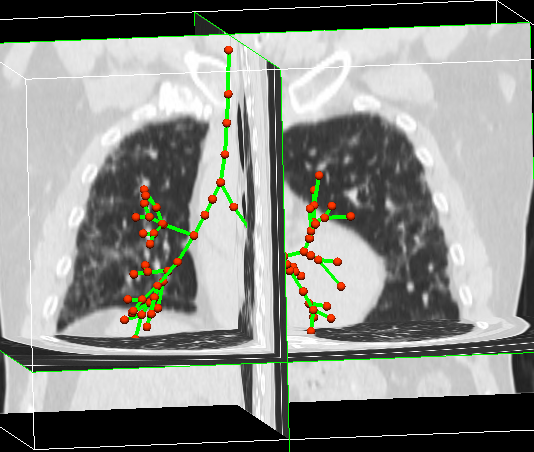
\includegraphics{ModelBasedAnalysis/Image/UpperAirwayDigitizing.png}}
  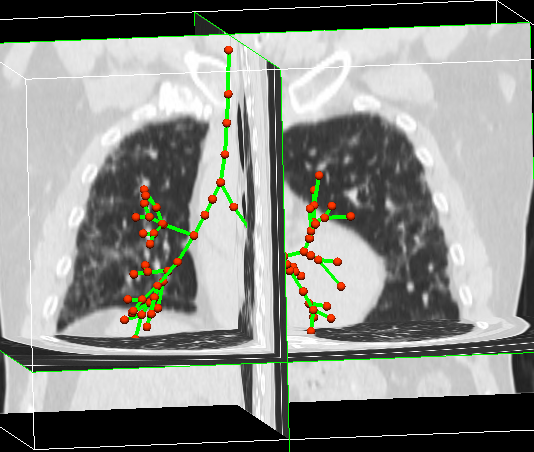
\includegraphics[width=\linewidth,trim={{.0\wd0} {.0\wd0} {.0\wd0} {.0\wd0}},clip]{ModelBasedAnalysis/Image/UpperAirwayDigitizing.png}
  \caption{Manual digitized upper airway}
  \label{fig:AirwayGeneration-a} 
\end{subfigure}
%\vspace{.1in} % control space between the upper context and figure
\hspace{.1in} % control space between two figures
\begin{subfigure}{.425\linewidth}% set image scale
  \sbox0{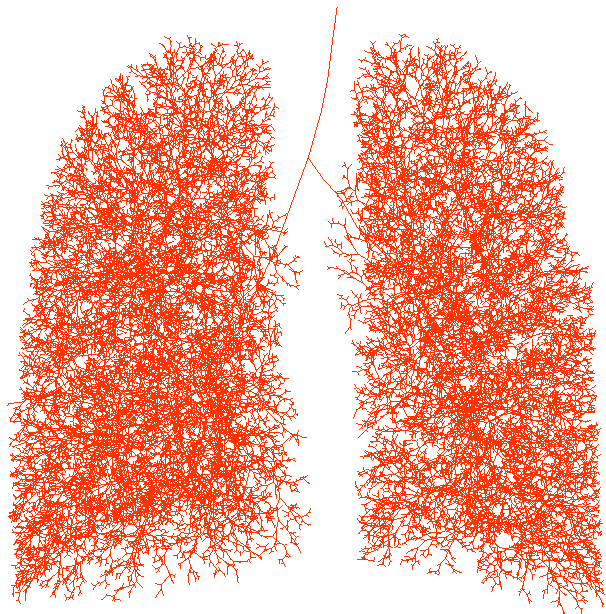
\includegraphics{ModelBasedAnalysis/Image/IPF511_Normal_FE_Airway.png}}
  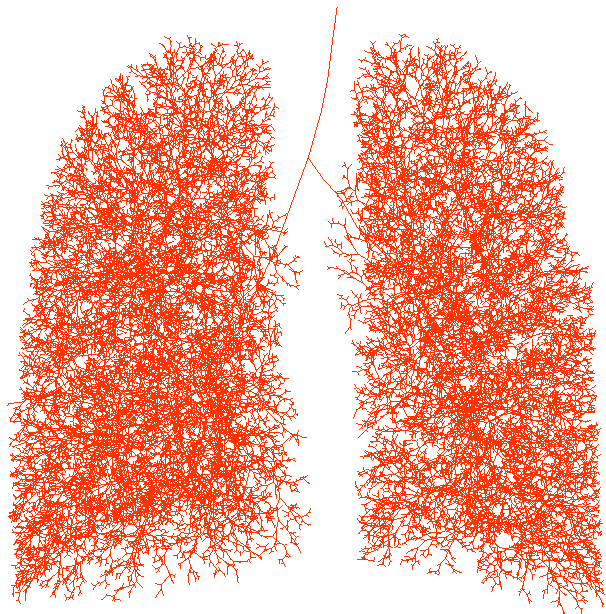
\includegraphics[width=\linewidth,trim={{.0\wd0} {.0\wd0} {.0\wd0} {.0\wd0}},clip]{ModelBasedAnalysis/Image/IPF511_Normal_FE_Airway.png}
  \caption{Full airway tree}
  \label{fig:AirwayGeneration-b} 
\end{subfigure}
\caption{Generation of airway tree. (a) Manual digitized upper airway tree from HRCT images in 3D. Blue lines are the centerlines of upper airway tree, and red points represent airway nodes. (b) Geometry of full conducting airway tree generated using volume-filling algorithm. The
model is shown from the anterior view, with the left lung on right, and right lung on left.} 
\label{fig:AirwayGeneration}
\end{figure}

In the next stage, the diameters of the airway branches were assigned for both IPF and control models. The method was:

1. The trachea radius for IPF was measured from segmented HRCT images (based on the segmented cross-section of larger airway branches) at 25\%, 50\%, and 75\% along the centreline of the trachea. The trachea radius was defined as the average of the three measurements.

2. The radius of the terminal bronchioles in the control models were assumed to be 0.2mm \citep{horsfield1976diameter}. The airways in the IPF lung have been found to be narrowed in 70\% of patients \citep{crystal1976idiopathic}. The terminal bronchiole radius for the IPF models was therefore scaled to a smaller value. The scaling was assumed to be in proportion to the ratio of IPF to control model volumes, as:

\begin{equation}
 \label{eq:NarrowedTerminalRadius}
 R_{{TB}_{IPF}} = R_{{TB}_{Control}} \times \sqrt[3]{\frac{FRC_{IPF}}{FRC_{Control}}},
\end{equation}

\noindent where $FRC_{IPF}$ is the measured FRC volume for the IPF patient and $FRC_{Control}$ is the reference FRC volume for the control model, $R_{{TB}_{IPF}}$ is the terminal bronchiole radius in the IPF models, and $R_{{TB}_{Control}}$ = 0.2mm is the terminal bronchiole radius in the reference (i.e. control) model.  

3. The radii of the other airway branches for the IPF models were calculated by assuming a constant Horsfield diameter ratio ($R_dH$) for each IPF subject. $R_dH$ is the rate of reduction of diameter (or radius) with reduction in Horsfield order, with $R_dH$ calculated by:

\begin{equation}
 \label{eq:HorsfieldRadiusRatio}
 R_dH = \frac{10 \times (\log_{10}R_{TB} - \log_{10}R_{Trachea})}{1-H_{Trachea}},
\end{equation}

\noindent where $R_{TB}$ is the terminal radius, $R_{Trachea}$ is the trachea radius, and $H_{Trachea}$ is the Horsfield order of the trachea.

4. While the $R_{TB}$ is expected to be smaller in IPF \citep{crystal1976idiopathic}, the anatomical deadspace ($V_D$) is actually larger \citep{plantier2016increased}. $R_{trachea}$ and $R_dH$ for the control models were therefore set such that $V_D$ (control) $<$ $V_D$ (IPF), for $R_{Trachea}$ within the normal published range for men (6.5-12mm) and women (5-11mm) \citep{breatnach1984dimensions}. $V_D$ (control) was initialized using $V_D$ (control) = $V_D$ (IPF) $\times (34.2/45.3)$, which is a relationship measured by \cite{plantier2016increased} for IPF and controls. $R_{Trachea}$ and $R_dH$ were adjusted until $R_{Trachea}$ was within the normal size range.

Using the above steps, a patient-specific pulmonary airway geometry for IPF and the control lung was constructed. 

\subsubsection{Vascular tree}
The centerlines of the first two generations of vessel trees were manually segmented from HRCT images, and represented as a 1-D finite element mesh. In this thesis, the pulmonary arterial and venous trees of other generations were assumed to be approximate replicas of the airway tree. Using the airway tree to approximate vessel geometry is a reasonable assumption, as the conventional pulmonary arteries generally follow the same branching pattern as the airways trees, and the airways and blood vessels have similar lengths and orientations. The airway and vasculature have been observed to bifurcate in union from larger branches to the bronchiole level, and the veins to divide at the approximate midpoint between adjacent airway bifurcations \citep{weibel1984pathway, hsia2016lung}. The manually-segmented main vessels plus the finite element model of the airway tree provided a full pulmonary blood vessel geometry for the IPF patient. The vascular structure for the control model was obtained using the same mapping procedure used for the airways as described previously. The microcirculatory model of \cite{clark2010contribution,clark2011interdependent} was appended to each terminal arteriole, to supply a corresponding terminal venule. This model is a symmetric-branching system of arterioles and venules that are connected (from arteriole to venule) at each generation by a recruitable and distensible ''capillary sheet''.

The unstrained (zero transmural pressure ($P_{tm}$)) radius of the main pulmonary artery ($R_{mArtery}$) and vein ($R_{mVein}$) were assigned based on the patient-specific (measured) trachea radius and data from morphometric studies (Equation \ref{eq:MainArteryRadius}and \ref{eq:MainVeinRadius}) \citep{horsfield1978morphometry,horsfield1981morphometry,huang1996morphometry}. The radius of all other arteries and veins down to the distal level were calculated based on a defined rate of increase in diameter with vessel Strahler order, the Strahler diameter ratio for artery and vein ($R_dS_{Artery}$ and $R_dS_{Vein}$). The value of $R_dS$ for the arterial tree and venous tree were specified according to the radius of the main artery and vein, and aiming for consistency with published human data \citep{horsfield1971models, horsfield1978morphometry,horsfield1981morphometry,huang1996morphometry}:

\begin{equation} 
 \label{eq:MainArteryRadius}
 R_{mArtery} = \frac{k_{Artery} \times R_{Trachea}}{{R_{Trachea_{ref}}}},
\end{equation}

\begin{equation} 
 \label{eq:ArteryStrahlerDiameterRatio}
 R_dS_{Artery} = \frac{10 \times (\log_{10}R_{sArtery} - \log_{10}R_{mArtery})}{1-S_{mArtery}},
\end{equation}

\begin{equation} 
 \label{eq:MainVeinRadius}
 R_{mVein} = 10 \times \log_{10}(\frac{k_{Vein} \times R_{Trachea}}{\log_{10}R_{Trachea_{ref}}}),
\end{equation}

\begin{equation} 
 \label{eq:VeinStrahlerDiameterRatio}
 R_dS_{Vein} = \frac{10 \times (\log_{10}R_{sVein} - \log_{10}(k_{Vein} \times R_{Trachea}))}{3 - S_{mArtery}},
\end{equation}

\noindent where $k_{Artery}$ is constant artery radius (equals to 11.53), $k_{Vein}$ is a constant for vein radius (equals to 6.3), $R_{Trachea_{ref}}$ is a statistical reference trachea radius (equals to 9 mm), $R_{sArtery}$ is the target for smallest arteries (equals to 0.125 mm), $R_{sVein}$ is the target for smallest veins (equals to 0.125 mm), and $S_{mArtery}$ is the Strahler order of the artery model. The vessel radius for the IPF models and the control models were then calculated. 
 
\subsection{Construction of computational models} \label{ComputationalModelConstruction}
In this chapter, computational modelling of lung function integrates previously published models of ventilation \citep{swan2012computational}, perfusion \citep{clark2010contribution, clark2011interdependent} and gas exchange \citep{clark2014lack} to simulate $\dot{V}/\dot{Q}$ distribution and oxygen and carbon dioxide exchange during tidal breathing in the upright posture. The patient-specific geometry of airways and vessels were used as input for these models. A brief introduction of the model components is summarized below, and details can be found in the referenced papers.

\subsubsection{Ventilation model}
The ventilation model developed by \cite{swan2012computational} was used to predict the time-averaged topological distribution of inhaled air in the upright human lung, governed by local tissue deformation, elastic recoil pressure, airway resistance and acinar compliance. Each of the acini in the tree model subtending each terminal bronchiole are assumed to function as compliant compartments. The acinar volume and compliance were initialised at FRC using a distribution of tissue strain along the gravitational direction that was consistent with strain computed by a tissue mechanics model \citep{tawhai2009supine}. The acinus volumes were perturbed around these values to provide variability as observed in the lung (a coefficient of variation of 0.1). Compliance of each acinus was calculated using a relationship between volume and compliance for isotropically expanding units of tissue in the \cite{tawhai2009supine} tissue mechanics model. Compliance C, is defined by

\begin{equation}
 \label{eq:TissueCompliance}
 C = [\frac{\xi e^{\gamma}}{6V_0}(\frac{3(3a+b)^2(\lambda^2-1)^2}{\lambda^2} + \frac{(3a+b)(\lambda^2 + 1)}{\lambda^4})]^{-1},
\end{equation}

\noindent where $\lambda$ is the (isotropic) stretch, $V_0$ is the undeformed volume, and $\gamma = \frac{3}{4}(3a+b)(\lambda^2-1)^2$. The movement of air into each acinar unit was determined by expansion of the alveolar tissue and airway resistance.

In this model, the flow through the conducting airways was assumed to be Poiseuille with a ''correction factor'' to account for additional energy losses that occur in branching airways \citep{pedley1970energy}. Additional energy losses caused by flow disturbances are created at the airway bifurcations and contribute to the calculation of pressure drop across the junction. A correction term, $Z_{Pe}$, was used to define the ratio of actual energy dissipation to Poiseuille flow dissipation, then the ratio of actual airway resistance ($R_{aw}$) to its Poiseuille flow equivalent ($R_P$) can be calculated by (ignoring kinetic energy changes):

\begin{equation}
 \label{eq:EnergyDissipation}
 Z_{Pe} = \frac{R_{aw}}{R_P} = \frac{K_{Pe}}{4\sqrt{2}}(R_e \times \frac{2r}{l})^{0.5},
\end{equation}

\noindent where $R_e$ is the Reynolds number, r and l are the radius and length of the airway, respectively. $R_e = \frac{2Q\rho}{\pi r \mu}$, where $\rho$ and $\mu$ are the density ($1.51 \times 10^{-6}g.mm^{-3}$) and viscosity ($1.92 \times 10^{-5}P_{a}.s$) of air, respectively. $K_{Pe}$ is a constant, set to 1.85. Then, the resistance of each airway branch was calculated as the Poiseuile resistance ($R_{aw}$) multiplied by the term $Z_{Pe}$, and the Poiseuille flow through each conducting airway was acquired by the following equation:

\begin{equation}
 \label{eq:PressureFlowEquation}
 P_{aw_2} - P_{aw_1} = R_{aw}\dot{V} = Z_{Pe}R_P\dot{V} = Z_{Pe}\frac{8l\mu}{\pi r^{4}}\dot{V},
\end{equation}

\noindent where $P_{aw_1}$, $P_{aw_2}$ are the air pressures at the start and end of a branch, and $\dot{V}$ is the air flow through the airway. The air flow into the acinus (modelled as a compliant unit subtending the terminal bronchiole) was determined by an equation of motion that relates airway resistance, air flow, tissue compliance and the rate of change of internal and external pressures:

\begin{equation}
 \label{eq:AcinarFlowEquation}
 P_{aw} = \frac{V_A}{C_A} + R_{aw}\dot{V} + I\frac{d\dot{V}}{dt} - P_l,
\end{equation}

\noindent where $P_{aw}$, $R_{aw}$ and $\dot{V}$ are the pressure, Poiseuille resistance and flow in the terminal bronchiole, $V_A$ and $C_A$ are the volume and compliance of the acinar unit, I is inertance of the unit, and $P_l$ is an external driving pressure (varied sinusoidally) working to expand the unit and drive air flow through the conducting airways to the terminal units.

Here, we assumed that the rate of change of airflow $\dot{V}$ is small enough, that the term $I\frac{d\dot{V}}{dt}$ in Equation \ref{eq:AcinarFlowEquation} can be neglected. A suitable small time interval, $\Delta t = t_n - t_{n-1}$, was defined, and the flow at the end of the time period $\dot{V}_n = \dot{V}(t_n)$ is:

\begin{equation}
 \label{eq:FlowRespectToTime}
 \dot{V}_n = C_A(\nu - \beta) + \dot{V}_{n-1} - C_A(\nu - \beta)exp(\frac{-\Delta t}{R_{aw}C_A}),
\end{equation}

\noindent where $\dot{V}_{n-1} = \dot{V}(t_{n-1})$ is the flow at the end of the previous time period. $\nu = dP_{aw}/dt$, and $\beta = dP_l/dt$ are the change of bronchiole pressure and driving pressure with respect to t, respectively. This equation is derived from Equation \ref{eq:AcinarFlowEquation}. The detailed description can be found in \cite{swan2012computational}.

\subsubsection{Perfusion model}
The pulmonary perfusion model developed by \cite{clark2011interdependent} was used to simulate a time-averaged distribution of blood flow, capillary blood volume and average \gls{rbc} transit time for each acinus unit. The full vascular structure (including arteries, veins, intra-acinar arterioles and venules, and capillaries) generated in Section \ref{AirwayVesselGeometry} was the geometric domain for this model. Distension of blood vessels and hydrostatic effects were also included in the model, with arterial and venous diameter and the thickness of the capillary sheet assumed proportional to the transmural pressure ($P_{tm}$). The intra-acinar (extra-capillary) blood flow was modeled in the symmetric ladder structure introduced previously. The microcirculatory model relates the vessel diameter, length and the thickness of capillary sheet.

Similarly to air flow, the flow through pulmonary arteries and veins was predicted using a Poiseuille equation, with an additional term for gravitational effects acting on blood in the vessels. The relationship is given by

\begin{equation}
 \label{eq:VesselFlow}
 \Delta P = P_{b2} - P_{b1} = \frac{128 \mu_bL\dot{Q}}{\pi D^{4}} + \rho_b Lgcos\theta,
\end{equation}

\noindent where $P_{b1}$ and $P_{b2}$ are the blood pressures at the beginning and end of the vessel element, $\mu_b$ and $\rho_b$ are the viscosity and density of the blood in the vessel, L and D are the vessel length and radius, $\dot{Q}$ is the volumetric flow rate in the vessel, g is the gravitational acceleration ($9.81m/s^2$), and $\theta$ is the angle between the vessel and the direction of gravity. 

The term $\rho_b Lgcos\theta$ in Equation \ref{eq:VesselFlow} represents the effect of gravity on blood in the vessels. In the microcirculatory model, an arteriole and venule were joined at each generation by a capillary bed, forming a ''ladder-like'' structure, to construct the intra-acinar circulation. Therefore, the term $\rho_b Lgcos\theta$ was considered negligible because the length of acinar arterioles and venules was assumed to be small enough, and

\begin{equation}
 \label{eq:VesselFlow1}
 \Delta P = \frac{128 \mu_bL\dot{Q}}{\pi D^{4}}.
\end{equation}

The strained diameter D in Equation \ref{eq:VesselFlow1} was assumed to have a linear relationship with the transmural pressure $P_{tm}$ as

\begin{equation}
 \label{eq:VesselDeformation}
 \frac{D}{D_0} = \alpha P_{tm} + 1,
\end{equation}

\noindent where $D_0$ is the unstrained vessel diameter, $\alpha$ is the vessel compliance constant. The tethering pressure acting on the blood vessel in the radial direction was assumed to be equal and opposite to the local tissue elastic recoil pressure ($P_e$), therefore $P_{tm} \approx P_b - P_e$, where $P_b$ is the average blood pressure along the vessel. Then, the blood flow through a capillary sheet ($\dot{Q}$) was modelled using the classic sheet flow theory developed by \cite{fung1969theory} as

\begin{equation}
 \label{eq:CapillarySheetFlow}
 \dot{Q} = \frac{SA}{\mu_c f l^{2}_{C}} \int\ H^{3}dP_{tm},
\end{equation}

\noindent where A is the alveolar surface area, S is the proportion of alveolar surface area (A) composed of capillaries, $\mu_c$ is the apparent viscosity of blood in the capillaries, f is the numerical friction factor, $l_C$ is the average path length through the capillary network between arteriole and venule. H is the thickness of the capillary sheet which was assumed to be approximately linearly dependent on $P_{tm}$ similar to Equation \ref{eq:VesselDeformation}

\begin{equation}
 \label{eq:CapillarySheetDeformation}
 \frac{H}{H_0} = \alpha_C P_{tm} + 1,
\end{equation}

\noindent where $H_0$ is the unstrained sheet thickness. In both Equation \ref{eq:VesselDeformation} and Equation \ref{eq:CapillarySheetDeformation}, maximum $P_{tm}$ was assumed to be $32 cmH_2 O(3.1KP_a)$. $\alpha_C$ is the compliance of the capillary sheet, which was assumed to reduce linearly with increase of transpulmonary pressure ($P_{tp}$)

\begin{equation} 
 \label{eq:CapillaryCompliance}
 \alpha_C(P_{tp}) = a + bP_{tp},
\end{equation}

\noindent where a and b are constants, $P_{tp}$ is assumed to be equal and opposite to $P_e$. The values of a and b were firstly measured for dogs by \cite{glazier1969measurements}, then scaled for human as a = 0.165$\mu m/cmH_2O$, b = -2.58$\mu m/{(cmH_2O)}^2$.

\subsubsection{Gas exchange model}
The ventilation and perfusion distribution predicted by the ventilation and perfusion models described in the previous section were used as inputs in a whole lung model of gas transport and exchange. The ventilation model provided the volume change in each acinus during inspiration and expiration. The perfusion model determined the acinar capillary blood volume and average RBC transit time. The modelling was based on the assumption that the acinus was well-mixed, and the ventilation and perfusion distributions were time-invariant. Then the rate of $O_2$ removal from the alveolar air and the rate of $CO_2$ transferred to the well-mixed alveolar compartment of the acinus were determined. The steady-state gas transfer model developed by \cite{kapitan1986computer} and used by \cite{clark2014lack} was used to predict the partial pressure of oxygen in alveolar air ($P_AO_2$) and in arterial blood ($P_aO_2$).

In each gas exchange acinar unit, the steady-state blood and gas compositions are related by conservation of mass. The equilibrium oxygen partial pressure was described through the relationship

\begin{equation} 
 \label{eq:SteadyStateEquation}
 \dot{V}_I P_{I_{O_2}} - \dot{V}_E P_{A_{O_2}} = k\dot{Q}_C(C_{C_{O_2}} - C_{\bar{V}_{O_2}}),
\end{equation}

\noindent where $\dot{V}_I$ is the unit's inspired ventilation (L/min), $P_{I_{O_2}}$ is the oxygen partial pressure (mmHg) of the humidified inspired air,  $\dot{V}_E$ is the expired (alveolar) ventilation (L/min), $P_{A_{O_2}}$ is the oxygen partial pressure (mmHg) of the alveolar air, k is a constant that accounts for differences in temperature and pressure between body and the atmosphere as well as allowing consistency between the units of the left and right hand side of Equation \ref{eq:SteadyStateEquation}, $\dot{Q}_C$ is the capillary blood flow, $C_{C_{O_2}}$ is the oxygen content in the end-capillary blood (ml gas/100 ml blood), and $C_{\bar{V}_{O_2}}$ is oxygen content entering the lungs from mixed venous blood (ml gas/100 ml blood). The $O_2$ and $CO_2$ contents are associated with the corresponding partial pressure of $O_2$ and $CO_2$ by the appropriate dissociation curve. The left-hand side of Equation \ref{eq:SteadyStateEquation} represents the volume rate of gas uptake from the compartment by the air, and the right-hand side represents the volume rate of gas uptake from the compartment by the blood. The rates are equal at steady-state.

The non-linear Monod-Wyman-Changeaux model \citep{monod1965nature} is used to solve the relationship between oxygen content and partial pressure. The oxygen content in the end-capillary blood $C_{C_{O_2}}$ in each acinus unit is related to the end-capillary oxygen partial pressure ($P_cO_2$) as

\begin{equation} 
 \label{eq:OxygenContent}
 C_{C_{O_2}} = \frac{15 \times 1.34 \times \rho(P_cO_2) + 0.03 \times P_cO_2}{100},
\end{equation}

\noindent where $\rho(P_cO_2)$ is the oxygen saturation, and it is a function of $P_cO_2$. The oxygen binding capacity with haemoglobin is 1.34 mL oxygen per gram of hemoglobin, and around 15 g of hemoglobin per 100 mL of blood. Therefore, the term $15 \times 1.34 \times \rho(P_cO_2)$ expresses oxygen bound to haemoglobin. The term $0.03 \times P_cO_2$ expresses the oxygen dissolved in blood plasma, which gives 0.03 mL of oxygen per 100 mL of whole blood for each mmHg of partial pressure.

The oxygen saturation $\rho(P_cO_2)$ was calculated from Monod-Wyman-Changeaux model \citep{monod1965nature} as

\begin{equation} 
 \label{eq:OxygenSaturation}
 \rho(P_cO_2) = \frac{LK_T \sigma P_cO_2 (1+K_T\sigma P_cO_2)^3 + K_R\sigma P_cO_2(1+K_R\sigma P_cO_2)^3}{L(1+K_T \sigma P_cO_2)^4 + (1+K_R \sigma P_cO_2)^4},
\end{equation}

\noindent where $K_R$ (equals to $3.6 \times 10^6 L/mol^{-1}$) and  $K_T$ (equals to $10 \times 10^3 L/mol^{-1}$) are the microscopic dissociation constants of a single ligand bound to a stereospecific site, in the two states (R and T), respectively. L (equals to $171.2 \times 10^6$) is the equilibrium constant for the state R to T transition, and $\sigma$ (equals to $1.4 \times 10^{-6} mol \cdot L^{-1}mm Hg^{-1}$) is the oxygen solubility.

In this model, it is assumed that the blood stays in the capillaries long enough to achieve equilibrium between the alveolar air and capillary blood, and $P_AO_2$ can equilibrate with $P_cO_2$ at the end of each inspiration. Therefore, $P_AO_2$ and $P_cO_2$ can be solved from Equation \ref{eq:SteadyStateEquation} using Newton’s method. The ventilation-weighted sum of $P_AO_2$ was calculated as an estimate of expired oxygen partial pressures from the full lung, and the perfusion-weighed sum of $C_cO_2$ was used to estimate the $P_aO_2$.

The predicted acinus ventilation and perfusion were used as input into the gas exchange model, and carbon dioxide transport was also simulated using the same assumption of equilibration between air and blood similar to the oxygen transfer model \citep{kapitan1986computer}. In each acinus unit, equilibration of carbon dioxide between air side and blood side was represented though a mass balance equation

\begin{equation} 
 \label{eq:CO2SteadyStateEquation}
 \dot{V}_A P_ACO_2 = k\dot{Q}_C(C_{C_{CO_2}} - C_{\bar{V}_{CO_2}}),
\end{equation}

\noindent where $\dot{V}_A$ is the expired or alveolar ventilation, $C_{C_{CO_2}}$ is the carbon oxygen content in the end-capillary blood, and $C_{\bar{V}_{CO_2}}$ is carbon oxygen content entering the lungs from mixed venous blood. As in the calculation for oxygen exchange, the assumption that transport time is sufficient to equilibrate between blood and air for carbon dioxide exchange was used, so that $P_ACO_2$ can be predicted by solving Equation \ref{eq:CO2SteadyStateEquation}. $P_cCO_2$ in each acinus unit was calculated from $C_{C_{CO_2}}$ using Henry’s law

\begin{equation} 
 \label{eq:CarbonOxygenContent}
 C_{C_{CO_2}} = \frac{M \cdot P_cCO_2}{1+M \cdot P_cCO_2}(P_cCO_2 - P_vCO_2),
\end{equation}

\noindent where M (equals to $23.86 ml \cdot mmHg^{-1}$) is the transfer factor for carbon oxygen across the capillary-alveolar membrane \citep{chakraborty2004diffusing}, and $P_vCO_2$ is the partial pressure of oxygen in mixed venous blood.

%An 1-D advection-diffusion equation was applied to model the gas transport through the conducting airway. The secondary flows in radial and circumferential directions were neglected here, thus the gas transport was solved in the axial direction along the airway branch at each time step:
%
%\begin{equation} 
 %\label{eq:AirSideGasTransport}
 %\frac{\partial c}{\partial t} + u_x \frac{\partial c}{\partial x} = D \frac{\partial^2c}{\partial x^2},
%\end{equation}
%
%\noindent where c is the gas concentration ($O_2$ or $CO_2$), x is the axial coordinate along the airway, $0 \leq x \leq L$ (L is the length of airway), $u_x$ is the axial velocity predicted by the ventilation model through conducting airway, D is the binary gas diffusion coefficient of gas. The advection-diffusion equation \ref{eq:AirSideGasTransport} was solved for each 1-D finite element of airway tree.
%
%The flow at the trachea (Q(0,t)) was set as a constant square waveform during a respiratory cycle:
%
%\begin{equation} 
 %\label{eq:TracheaFlow}
 %Q(0,t) = \begin{cases}
 %0.16Ls^{-1} \quad\quad during \quad inspiration\\
 %-0.16Ls^{-1} \quad during \quad expiration
 %\end{cases}
%\end{equation}
%
%During inspiration, a zero flux was applied to the end of each terminal bronchiole as boundary condition. During expiration, the terminal bronchiole concentration (c(L,t)) was set to be equal to the mixed acinar concentration ($c_A$):
%
%\begin{equation} 
 %\label{eq:TerminalBoundaryCondition}
 %\begin{split}
 %\frac{dc(L,t)}{dx} = 0 \quad during \quad inspiration, \\
 %c(L,t) = c_A \quad during \quad expiration,
 %\end{split}
%\end{equation}
%
%\noindent where x = 0 and x = L represent the location of trachea and terminal bronchioles. The volume change of acinar unit during each time step ($dV_A$) during respiratory cycle was acquired by:
%
%\begin{equation} 
 %\label{eq:StepAcinarVolumeChange}
 %dV_A = Q(0,t)\dot{V_A}\Delta t,
%\end{equation}
%
%\noindent where $\dot{V_A}$ is the proportional ventilation received for that acinar unit to the total lung ventilation, $\Delta t$ is the time step. Therefore, the updated acinar volume at the $n^{th}$ time step can be represented as: $V_{A(n)} = V_{A(n-1)} + dV_A$.
%
%Acinar concentration ($c_{A(n)}$) was updated with the inspired air into the acinar unit during inspiration, and with the gas exchange flux during expiration:
%
%\begin{equation} 
 %\label{eq:TracheaFlow}
 %C_{A(n)} = \begin{cases}
 %\frac{(c_{A(n-1)}V_{A(n-1)} + n_{insp}) + n_{exch}}{V_{A(n)}} \quad during \quad inspiration\\
 %\frac{(c_{A(n-1)}V_{A(n-1)} + n_{exch}}{V_{A(n)}} \quad\quad\quad during \quad expiration
 %\end{cases}
%\end{equation}
%
%\noindent where $n_{insp} = dV_A c(L,t)$ is the mass of inspired $O_2$ or $CO_2$. $n_{exch} = q_A \Delta t$ is the mass of $O_2$ or $CO_2$ exchanged with the capillary blood, where $q_A$ is the gas exchange flux for $O_2$ or $CO_2$.
%
%The exchange of $O_2$ in an acinar unit was predicted at each time step using the model developed by \cite{ben2006simplified, swan2010evidence, swan2010multi}:
%
%\begin{equation} 
 %\label{eq:O2ExchangeEquation}
 %\frac{dP_aO_2}{dt} = \frac{T_{tO_2}}{\sigma_{O_2} V_b}{(1 + \frac{4[Hb]_b}{\sigma_{O_2}}\frac{dS_{O_2}}{dP_a O_2})}^{-1} \times (P_A O_2 - P_a O_2),
%\end{equation}
%
%\noindent where $P_a O_2$ and $P_A O_2$ are oxygen partial pressure in alveolar and in arterial blood, respectively. $\sigma_{O_2}$ is the $O_2$ diffusion coefficient, $V_b$ is the capillary blood volume, $[Hb]_b$ is the concentration of haemoglobin in blood, $S_{O_2}$ is the slope of the oxyhaemoglobin dissociation curve. $T_{tO_2}$ is the oxygen transfer factor which represents the ability of transferring $O_2$ from lungs into capillary blood by:
%
%\begin{equation} 
 %\label{eq:O2TransferFactor}
 %T_{tO_2} = ((\frac{\eta\phi S_A}{\tau_h})^{-1} + (V_b \theta_{O_2})^{-1})^{-1},
%\end{equation}
%
%\noindent where $S_A$ is the alveolar air surface area in an acinus available for exchange and is assumed to be equal for all acinus. $\tau_h$ is the total membrane thickness, $\eta$ and $\phi$ are constants. $\theta_{O_2}$ is the rate of $O_2$ uptake by the whole blood which is determined by:
%
%\begin{equation} 
 %\label{eq:OxygenUptakeRate}
 %\theta_{O_2} = \acute{k}_c \sigma_{O_2}(1 - S_{O_2})k[Hb]_b,
%\end{equation}
%
%\noindent where $\acute{k}_c$ is the forward reaction velocity for $O_2$ binding to haemoglobin, k is the capacity of $O_2$ carrying haemoglobin, $S_{O_2}$ is the oxyhaemoglobin saturation. The details of the calculation of $S_{O_2}$ can be found in \cite{swan2010evidence, swan2010multi}.
%
%The exchange of $CO_2$ was predicted using a simplified model by describing the bicarbonate ($HCO^{-}_3$) hydration-dehydration reaction to produce $CO_2$ and $H_2 O$. The change rate of arterial partial pressure of $CO_2$ ($P_a CO_2$) was determined by the amount of $CO_2$ for exchanging between capillary blood and alveolar air. The $CO_2$ formed from hydration-dehydration reaction:
%
%\begin{equation} 
 %\label{eq:CO2ExchangeEquation}
 %\frac{dP_a CO_2}{dt} = \frac{T_{tCO_2}}{\sigma_{CO_2}V_b}(P_A CO_2 - P_a CO_2) - \delta k_u P_b CO_2 + \delta \frac{k_v}{\sigma_{CO_2}K}[H]^{+}[HCO^{-}_3],
%\end{equation}
%
%\noindent where $P_A CO_2$ is the alveolar partial pressure of $CO_2$. $k_u$ is $CO_2$ hydration constant, $k_v$ is constant of $HCO^{-}_3$ dehydration velocity constant, and $\delta$ is a fitted constant of $CO_2$ hydration reaction acceleration rate. The $CO_2$ solubility coefficient $\sigma_{CO_2}$ describes the capacity of carrying $CO_2$, $[HCO^{-}_3]$ and $[H]^{+}$ are the bicarbonate and hydrogen ion concentrations respectively. $T_{tCO_2}$ is $CO_2$ transfer factor which measures the capability to transfer $CO_2$ from capillary blood to the lungs:
%
%\begin{equation} 
 %\label{eq:CO2TransferFactor}
 %T_{tCO_2} = ((20 \times T_{MO_2})^{-1} + ({\frac{ln(2)\sigma_{CO_2}}{t_{\frac{1}{2}RBC}(1/V_p + 1/V_r)}}^{-1}))^{-1},
%\end{equation}
%
%\noindent where $T_{MO_2} = (\frac{\mu\phi S_A}{\tau_h})^{-1}$ is the membrane transfer factor for $O_2$ which equals to the first term of Equation \ref{eq:O2TransferFactor}. $V_p$ and $V_r$ are the volumes occupied by RBC and plasma respectively, which determines the RBC transfer factor component. $t_{\frac{1}{2}RBC}$ is the half time of equilibration of $CO_2$ across the erythrocyte membrane measured from experiment.

Some parameter values used in the ventilation, perfusion and gas exchange models are listed in Table \ref{tab:ModelParameters}. More details of the models are given in \cite{swan2010evidence}, \cite{swan2010multi}, \cite{clark2011interdependent}, and \cite{swan2012computational}.

%\newgeometry{bottom=1cm, top=1cm, left=0.5cm, right=0.5cm} %set the left margin of page
%\begin{landscape}
\newcolumntype{C}[1]{>{\centering\arraybackslash}p{#1}}
\begin{table}[htbp]
\centering
\caption{Parameter values and their source used in computational models}
\label{tab:ModelParameters}
\begin{tabular}{p{2.0cm} p{4.5cm} p{3.8cm} p{3.2cm}}
\hline
\bf{Parameter} & \bf{Description} & \bf{Value} & \bf{Source} \\ 
\hline
$K_{Pe}$ & Pedley correction factor & 1.85 & \cite{pedley1970energy} \\
$p$ & Air density & $1.15 \times 10^{-6}g.mm^{3}$ & Ideal gas law (37C) \\
$\mu$ & Air viscosity & $1.92 \times 10^{-6}$ & Sutherland's formula (37C) \\
$\alpha$ & Vessel compliance & $1.49 \times 10^{-4}Pa^{-1}$ & \cite{krenz2003flow} \\
$\mu_b$ & Blood viscosity & $3.36 \times 10^{-3}Pa/s$ & \cite{pries1996biophysical} \\
$p_b$ & Blood density & $1.05 \times 10^{-6}kg/mm^{3}$ & \cite{pries1996biophysical} \\
$\mu_c$ & Apparent viscosity of blood in capillary bed & $1.92 \times 10^{-3}Pa/s$ & \cite{fung2013biomechanics} \\
$f$ & Numerical friction factor & 21.6 & \cite{fung2013biomechanics} \\
$\alpha_c$ & Compliance of capillary sheet & $1.30 \times 10^{-9}Pa/s$ & \cite{fung1969theory} \\
$l_c$ & Pathlength from arteriole to venue & $11.86 \times 10^{-6}m$ & \cite{clark2010contribution} \\
$K_R$ & microscopic dissociation constant & $3.6 \times 10^6 L/mol^{-1}$ & \cite{monod1965nature} \\
$K_T$ & microscopic dissociation constant & $10 \times 10^3 L/mol^{-1}$ & \cite{monod1965nature} \\
L & equilibrium constant & $171.2 \times 10^6$ & \cite{monod1965nature} \\
$\sigma$ & oxygen solubility & $1.4 \times 10^{-6} mol \cdot L^{-1}mm Hg^{-1}$ & \cite{monod1965nature} \\
M & transfer factor for carbon oxygen across the capillary-alveolar membrane & $23.86 ml \cdot mmHg^{-1}$ & \cite{chakraborty2004diffusing} \\
%$[Hb]_b$ & Haemoglobin concentration in blood & $2.33mM$ & \cite{hall2015guyton} \\
%$S_A$ & Alveolar surface area of the lung & $130 \times 10^{4}cm^{2}$ & \cite{weibel2005design} \\
%$\eta$ & Krogh's permeation coefficient for $O_2$ & $5.5 \times 10^{-10}cm^{2}s^{-1}mmHg^{-1}$ & \cite{weibel1993morphometric} \\
%$\phi$ & Correction factor for surface folds & $0.8$ & \cite{weibel1993morphometric} \\
%$\tau_h$ & Harmonic mean thickness of the air-blood barrier & $1.11 \times 10^{-4}cm$ & \cite{weibel1993morphometric} \\
%$\acute{k}_c$ & Forward reaction velocity $O_2-Hb$ binding & $4.4 \times 10^{2}mM^{-1}s^{-1}$ & \cite{weibel1997design} \\
%$\sigma_{O_2}$ & $O_2$ solubility coefficient & $1.4 \times 10^{-3}mM \quad mmHg^{-1}$ & \cite{keener1998mathematical} \\
%$\sigma_{CO_2}$ & $CO_2$ solubility coefficient & $3.5 \times 10^{-2}mM \quad mmHg^{-1}$ & \cite{keener1998mathematical} \\
%$t_{\frac{1}{2}RBC}$ & Half-time of equilibration for $CO_2$ diffusion & $0.0001 s$ & \cite{hill1973mathematical} \\
%$k_u$ & $CO_2$ hydration velocity constant & $0.12s^{-1}$ & \cite{hill1973mathematical} \\
%$k_v$ & $HCO^{-}_3$ dehydration velocity constant & $89s^{-1}$ & \cite{hill1973mathematical} \\
%$\delta$ & $CO_2$ hydration reaction acceleration rate & $10^{1.9}$ & \cite{ben2006simplified} \\
\hline
\end{tabular}
\end{table}
%\end{landscape}
%\restoregeometry

\subsection{Modelling lung function}
Ventilation, perfusion and gas exchange models were solved under normal conditions (using lung and airway geometry for older normal people) and diseased conditions (using lung and airway geometry of IPF patients). Individual subject tissue classification from CALIPER was projected to the IPF airway/vessel trees as labelled disease regions to drive the patient-specific functional modelling of IPF, with fibrosis reducing tissue compliance and narrowing vessel radius. The subject-specific tidal volume, cardiac output, oxygen consumption ($\mathrm{VO_2}$) and carbon dioxide consumption ($\mathrm{VCO_2}$) were estimated based on the patient's individual information. Data from PFTs (introduced in Section \ref{ClinicalData}) were used as boundary conditions to control the simulations.

\subsubsection{Disease region labelling}
The different tissue patterns classified by CALIPER were mapped to the individual airway/vessel trees of each subject. For each airway/vessel terminal node, the corresponding tissue pattern it belonged to (is surrounded by) was extracted through finding the tissue pattern of the closest voxel to the node, so that each terminal node can be indexed to a particular tissue pattern. The percentage distribution of each tissue pattern against gravitational height (cranio-caudal axis) quantified in Chapter 4 was also used in the labelling. If the initial labelled amount of disease nodes was less than the cranio-caudal percentage, additional disease regions were added until the cranio-caudal distribution of disease matched the CALIPER classified data. Figure \ref{fig:DiseaseLabeling} shows the disease labelled airway nodes of one patient diagnosed with IPF. Table \ref{tab:DiseasePercent} lists the volume percentage of fibrosis (honeycomb + reticular + ground-glass) and emphysema classified by CALIPER software for each time point of these two patients.

\begin{figure}[htbp] 
\centering
\begin{subfigure}{.39\linewidth}% set image scale
  \sbox0{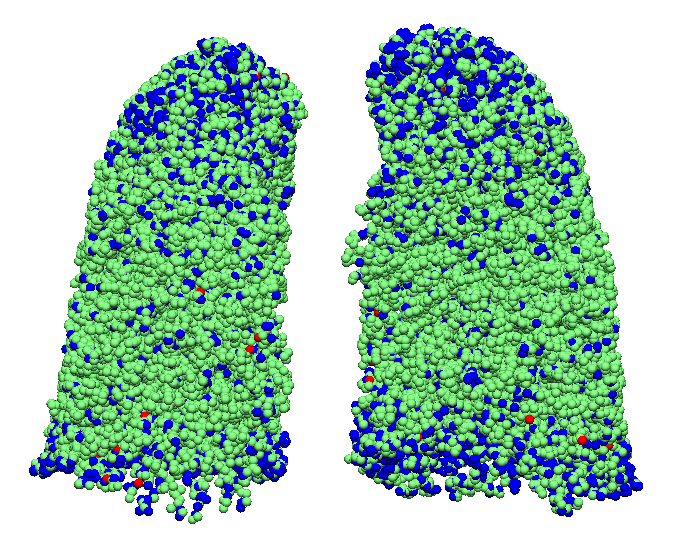
\includegraphics{ModelBasedAnalysis/Image/IPF501_DiseaseDistribution_vs_Height.png}}
  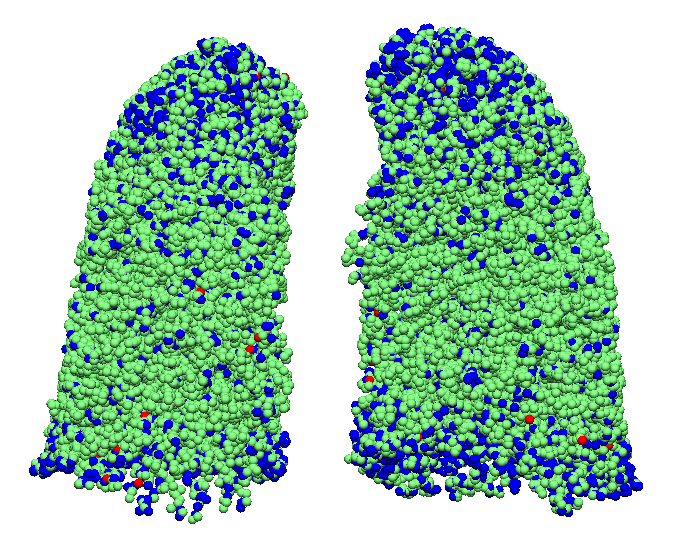
\includegraphics[width=\linewidth,trim={{.0\wd0} {.0\wd0} {.0\wd0} {.0\wd0}},clip]{ModelBasedAnalysis/Image/IPF501_DiseaseDistribution_vs_Height.png}
  \caption{Disease labelled airway nodes}
  \label{fig:DiseaseLabeling-a} 
\end{subfigure}
%\vspace{.3in} % control space between the upper context and figure
\hspace{.5in} % control space between two figures
\begin{subfigure}{.51\linewidth}% set image scale
  \sbox0{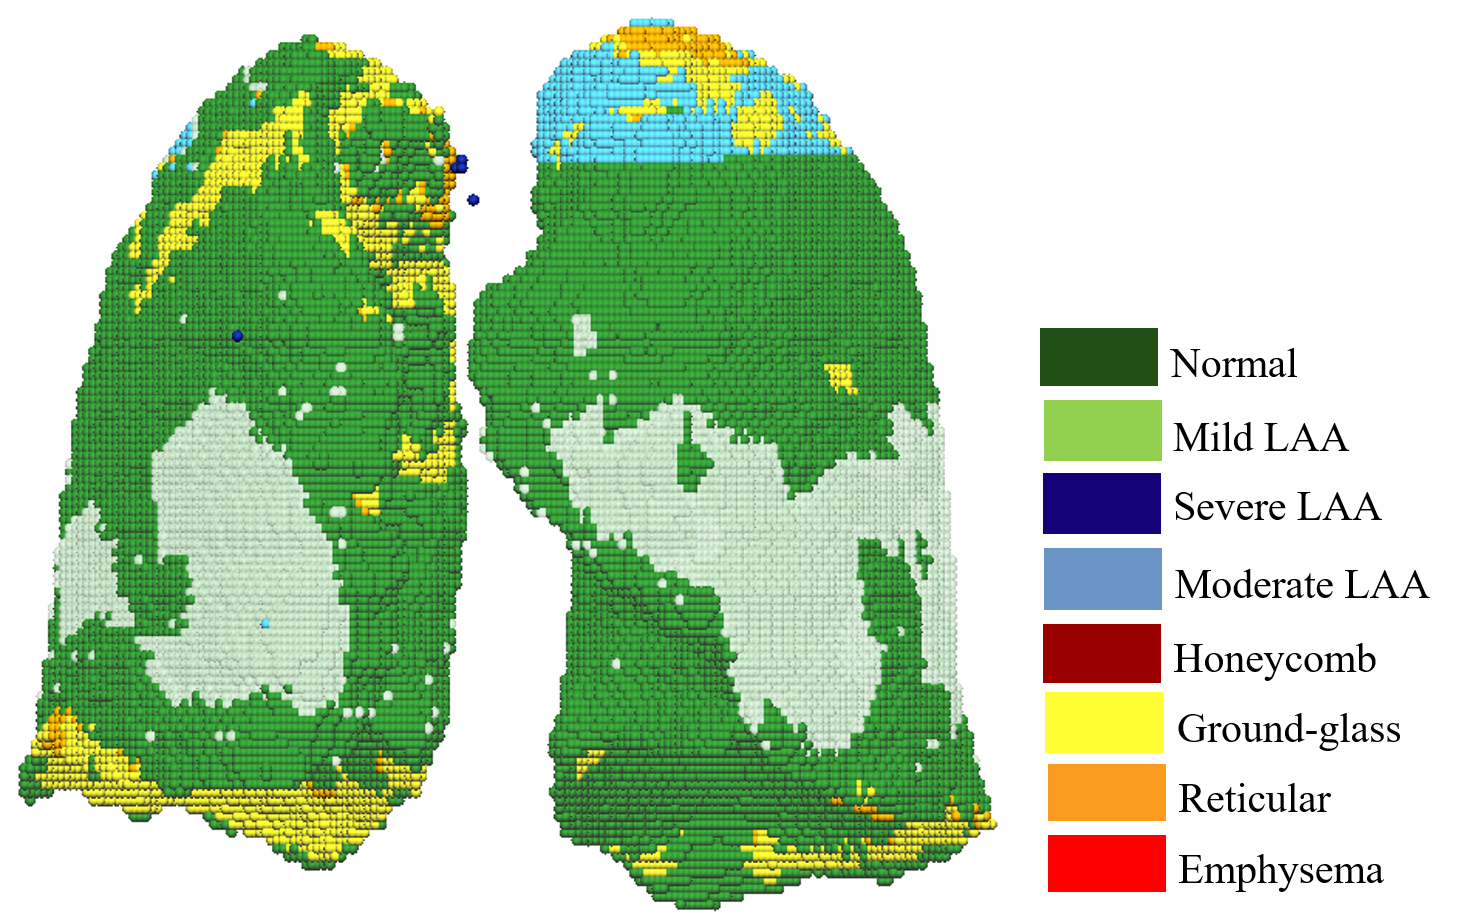
\includegraphics{ModelBasedAnalysis/Image/IPF501_CAPLIPERClassifiedData_colorbar.png}}
  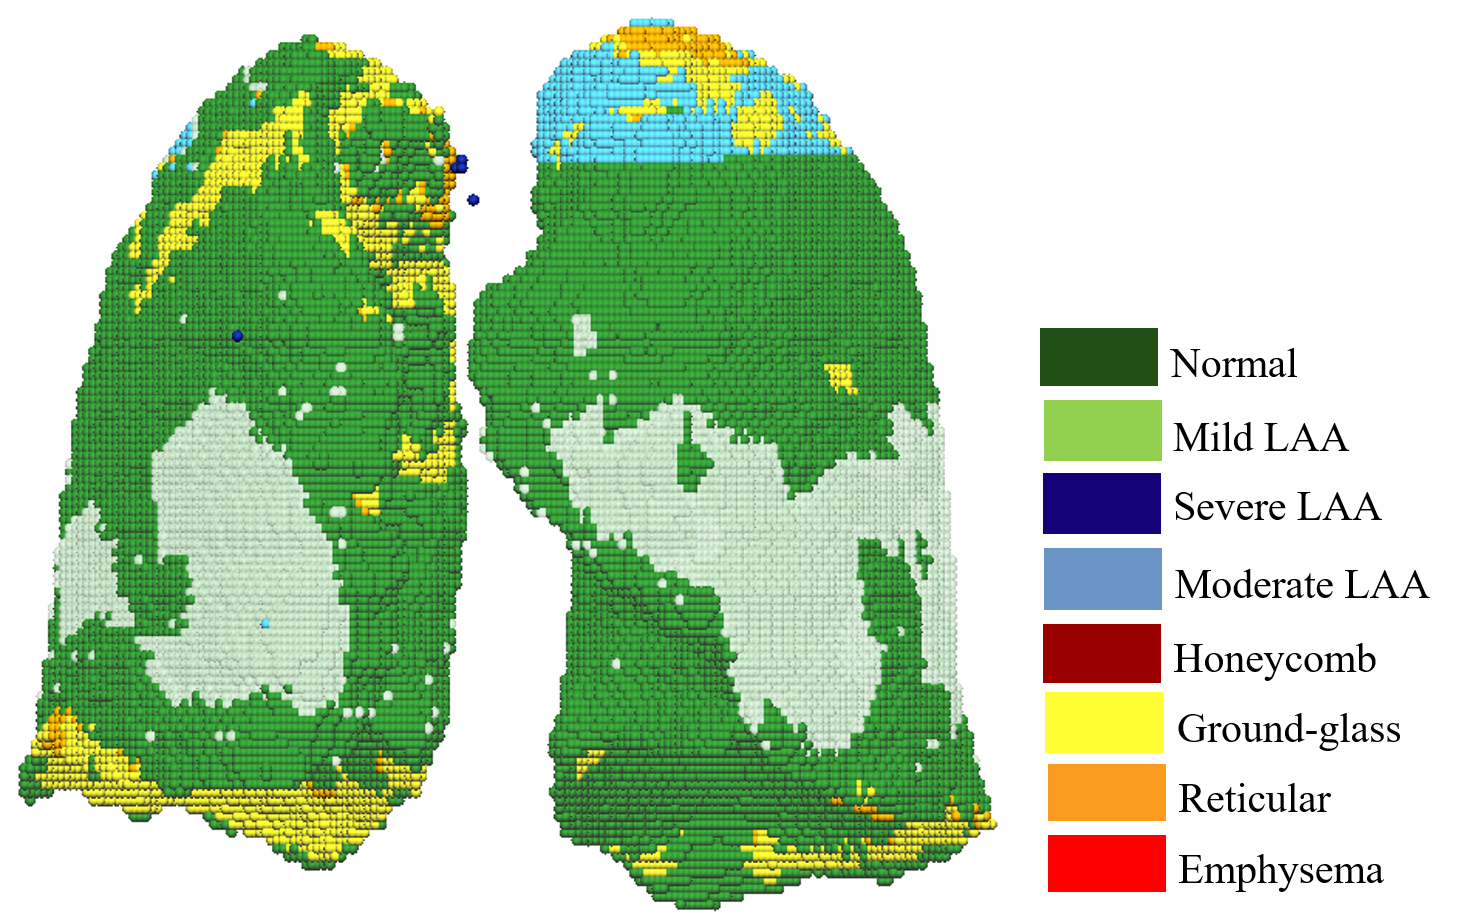
\includegraphics[width=\linewidth,trim={{.0\wd0} {.0\wd0} {.0\wd0} {.0\wd0}},clip]{ModelBasedAnalysis/Image/IPF501_CAPLIPERClassifiedData_colorbar.png}
  \caption{CALIPER classified tissue patterns}
  \label{fig:DiseaseLabeling-b} 
\end{subfigure}
\caption{Disease labeled airway nodes. For the model in (a), green is classified as normal tissue, blue is fibrosis, and red is emphysema. For the classified data in (b), the colour scheme indicates the tissue classification type}
\label{fig:DiseaseLabeling}
\end{figure}

%\begin{figure*}[htbp]
  %\centering 
  %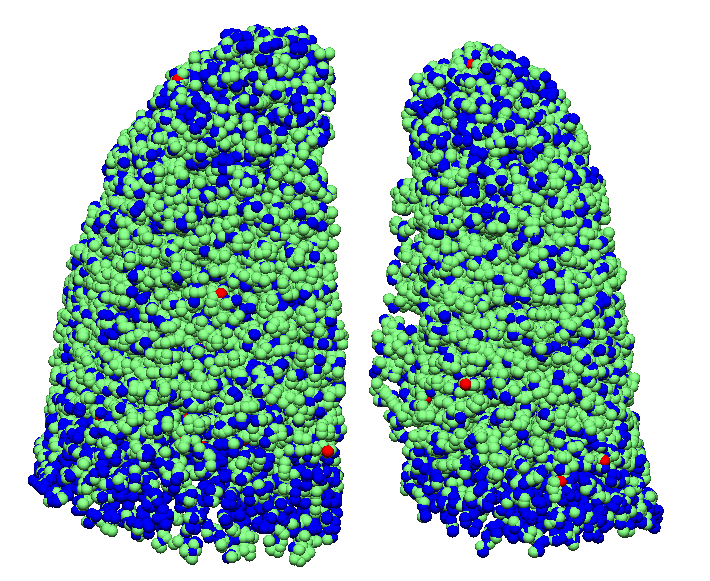
\includegraphics[height=2.9in]{ModelBasedAnalysis/Image/IPF501_DiseaseDistribution_BasedVentilation.png}
  %\caption{Disease labeled airway nodes. Green is classified as normal tissue, blue is fibrosis, and red is emphysema.}
  %\label{fig:DiseaseLabeling}
%\end{figure*}

\begin{table}[htbp]
\centering
\caption{The volume percentage of CALIPER classified disease tissues for each time point of these two patients (\%).}
\label{tab:DiseasePercent}
%\begin{tabular}{| c | c | c | c | c | c | c |}
\begin{tabular}{| p{1.6cm} | p{2.2cm} | p{2.0cm} | p{1.8cm} | p{1.8cm} | p{1.8cm} | p{2.1cm} |}
\hline
\bf{Patient No.} & \bf{Time point} & \bf{Honeycomb} & \bf{Reticular} & \bf{Ground-glass} & \bf{Total fibrosis} & \bf{Emphysema}\\ 
\hline
\multirow{2}*{Patient 1} & Time point 1 & $<$ 1\% & 6.78 & 8.84 & 15.62 & $<$ 1\%\\	
\cline{2-7}
~ & Time point 2 & $<$ 1\% & 4.13 & 13.62 & 17.77 & $<$ 1\%\\
\cline{2-7}
~ & Time point 3 & $<$ 1\% & 3.53 & 13.05 & 16.60 & $<$ 1\%\\			
\hline
\multirow{2}*{Patient 2} & Time point 1 & $<$ 1\% & 1.96 & 2.42 & 4.38 & $<$ 1\%\\	
\cline{2-7}
~ & Time point 2 & $<$ 1\% & 4.12 & 8.58 & 12.72 & $<$ 1\%\\	
\hline
\end{tabular}
\end{table}

\subsubsection{Deep inspiration model} 
To determine an appropriate total compliance for the IPF model, the model was required to predict the patient's forceful inhalation from FRC to TLC. Inhalation muscle pressure was assumed to be the same in normal and IPF, therefore an appropriate muscle pressure was estimated for the normal model and used in the IPF model. A deep inspiration model was constructed based on the ventilation model (introduced in Section \ref{ComputationalModelConstruction}) to simulate a deep inspiration from FRC to TLC. For simulation in the control models, the reference FRC volume (that is the patient-specific predicted normal volume as reference) from PFTs was used as an initial volume to start inspiration, and a subject-specific muscle pressure was solved to drive the lung expansion to the target reference TLC volume (the predicted TLC for the patient). Under the assumption that inspiratory muscle strength does not change with IPF disease \citep{de1980inspiratory}, the same driving pressure was used to simulate a deep inspiration in the corresponding IPF model. The IPF models started from their measured FRC. The modelling for IPF patients was divided into two separate stages:

1. The compliance of acini in labelled fibrosis regions (sum of honeycomb, reticular and ground-glass) was reduced to a very low value (less than 0.001 $\mathrm{L/cmH_2O}$) to represent stiffness due to fibrosis. Then, inspiration was modelled under this initial fibrosis condition.

2. The deep inspiration volume for IPF models acquired in Step 1 was used as the target volume, and the tissue compliance of every acinar unit was scaled down together until the simulated inspiration volume can hit the target, then the corresponding scale factor of total tissue compliance was acquired.

\subsubsection{Passive ventilation model}
Time-averaged passive ventilation to each acinus over four breathing cycles was predicted using the previously described ventilation model. Acinar volumes in the control and IPF models were initialized to FRC, using the reference normal value and measured disease value, respectively. The scale factor for acinar tissue compliance identified in Step 2 (above) was applied in the simulation for the IPF patient. Patient-specific tidal volume was estimated based on the patient's weight, gender and height \citep{gilbert1972changes, pelosi1998effects}.

\subsubsection{Perfusion model}
The perfusion model introduced in Section \ref{ComputationalModelConstruction} was used to estimate the distribution of blood. The individual age, weight, height and gender were used to predict the cardiac output for each patient \citep{brandfonbrener1955changes, miyamura1973maximum, stelfox2006hemodynamic}, and the inlet and outlet pressure were adjusted in order to match the estimated cardiac output. Based on previous observations of reduced perfusion in regions of fibrosis \citep{crystal1976idiopathic, strickland1993cause, plantier2018physiology}, the blood vessel radius in the fibrosis labelled regions were narrowed for IPF models, so that the blood flow would be reduced to the abnormal tissue.

\subsubsection{Gas exchange model}
The gas transport and exchange were simulated using the gas exchange model introduced in Section \ref{ComputationalModelConstruction}. The ventilation and perfusion distribution predicted by the ventilation and perfusion model were used as inputs in the normal and disease condition. Patient-specific oxygen consumption ($\mathrm{VO_2}$) and carbon dioxide consumption ($\mathrm{VCO_2}$) were estimated using the following equations \citep{kwan2004standard, coelho2013estimation}:

\begin{equation} 
 \label{eq:O2ConsumptionEstimation}
 VO_2 = P_{VO_2} \times W,
\end{equation}

\begin{equation} 
 \label{eq:CO2ConsumptionEstimation}
 VCO_2 = VO_2 \times 0.8,
\end{equation}

\noindent where $P_{VO_2}$ is the oxygen consumption at rest ($P_{VO_2} = 2.84 \pm 0.34 ml/kg^{-1}/min^{-1}$ for male and $P_{VO_2} = 2.82 \pm 0.37 ml/kg^{-1}/min^{-1}$ for female), and W is the weight of the patient (kg).

Using the patient-specific (or control-specific) tidal volume and dead space, and patient- (or control-) specific distribution of $\dot{V}$ and $\dot{Q}$, the partial pressure of oxygen in alveolar ($P_AO_2$) and in arterial blood ($P_aO_2$) can be predicted using the Kapitan \& Hempleman gas transfer model \citep{kapitan1986computer}.
\newpage

%%%%%%%%%%%%%%%%%%%%%%%%%%%%%%%%%%%%%%%%%%%%%%%%%%%%%%%%%%%%%%%%%%%%%%
\section{Results}
\subsection{Construction of lung lobe geometry}
Table \ref{tab:PatientIndividualData} lists the age, BMI and functional measures used for normal control lung shape prediction for one patient with IPF. The values for FVC, TLC, RV/TLC, and DLCO were predicted reference values from the patient's individual information. Figure \ref{fig:LungShapePrediction} presents the lung mesh of the IPF patient and its corresponding predicted control lung mesh for the matching normal. 

The lobe volume proportions for IPF lung meshes and predicted control meshes are shown in Table \ref{tab:AverageLobeVolume_Predicted}. As discussed in Chapter 4, Section \ref{SSMBasedAnalysis}, the shape change in IPF usually relates to a relatively larger anterior-posterior diameter and smaller height of the lung. The IPF lung has a lower average volume proportion for the left lower lobe and right lower lobe compared with normal older subjects. The results illustrated in Figure \ref{fig:LungShapePrediction} and Table \ref{tab:AverageLobeVolume_Predicted} are consistent with these previous findings, with the predicted lung mesh for normal controls showing a ''thinner'' and ''elongated'' shape and lower average volume of left and right lower lobes compared with the IPF mesh generated from CT imaging.

\begin{table}[htbp]
\centering
\caption{Predicted reference values used as input to predict a shape model for a normal control.}
\label{tab:PatientIndividualData}
\begin{tabular}{| l | c | c| c | c| c | c|}
\hline
\bf{Parameters} & \bf{Age} & \bf{BMI} & \bf{FVC(L)} & \bf{TLC(L)} & \bf{RV/TLC} & \bf{DLCO(mL/mmHg/min)}\\
\hline 
\bf{Values} & 82 & 32.77 & 3.87 & 7.22 & 46 & 25.1\\
\hline
\end{tabular}
%\begin{tablenotes}
  %\item[1] FVC, TLC, RV/TLC and DLCO are the patient-specific normal reference values acquired from PFT results.
%\end{tablenotes}
\end{table}

\begin{figure}[htbp] 
\centering
\begin{subfigure}{.49\linewidth}% set image scale
  \sbox0{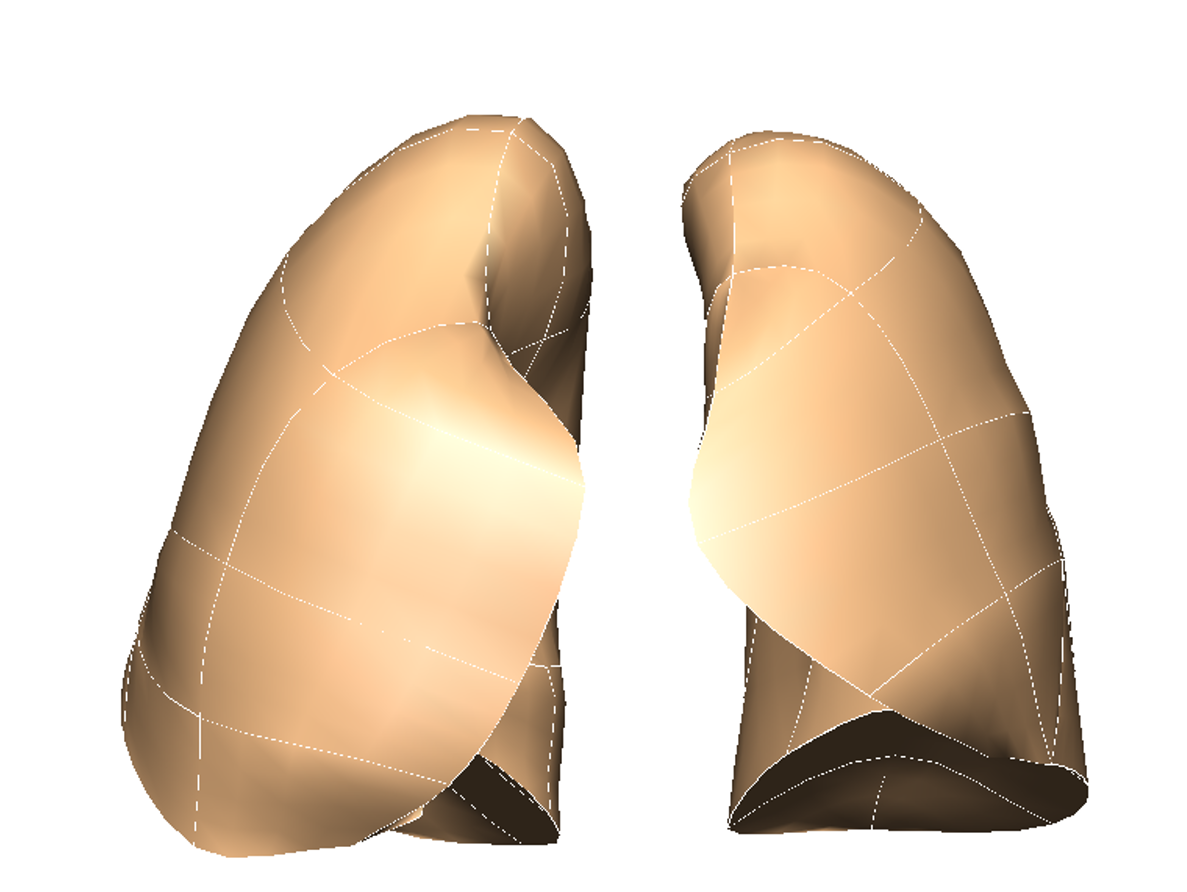
\includegraphics{ModelBasedAnalysis/Image/IPF405_IPFLungMesh.png}}
  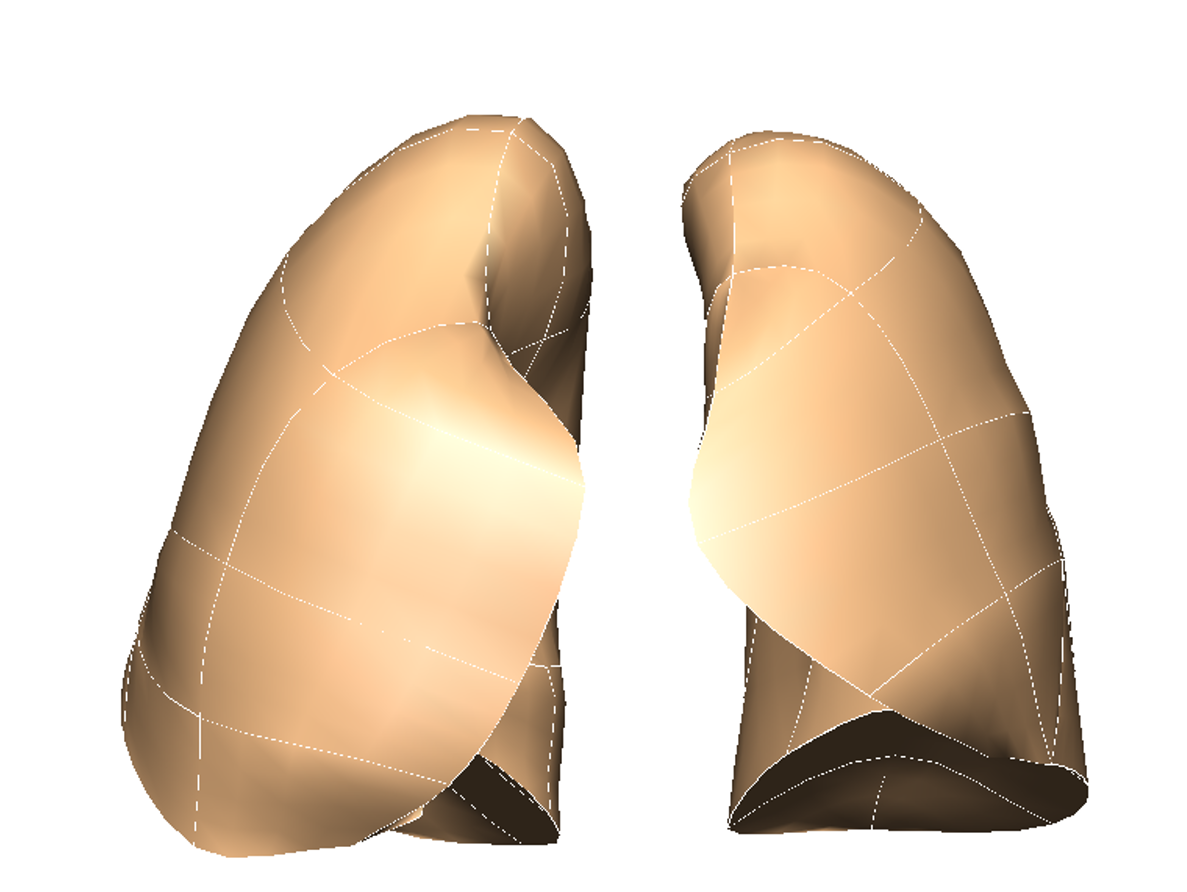
\includegraphics[width=\linewidth,trim={{.0\wd0} {.0\wd0} {.0\wd0} {.0\wd0}},clip]{ModelBasedAnalysis/Image/IPF405_IPFLungMesh.png}
  \caption{IPF lung mesh}
  \label{fig:LungShapePrediction-a} 
\end{subfigure}
%\vspace{.3in} % control space between the upper context and figure
\hspace{.4in} % control space between two figures
\begin{subfigure}{.4\linewidth}% set image scale
  \sbox0{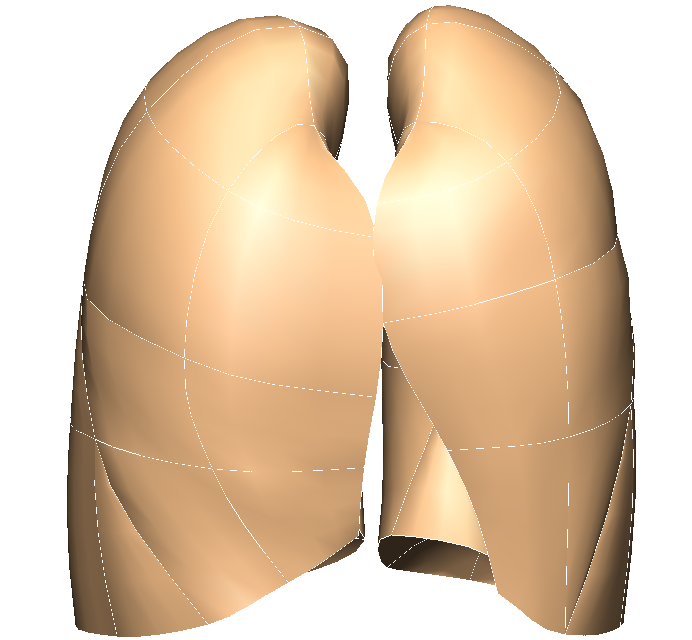
\includegraphics{ModelBasedAnalysis/Image/IPF405_NormalLungMesh.png}}
  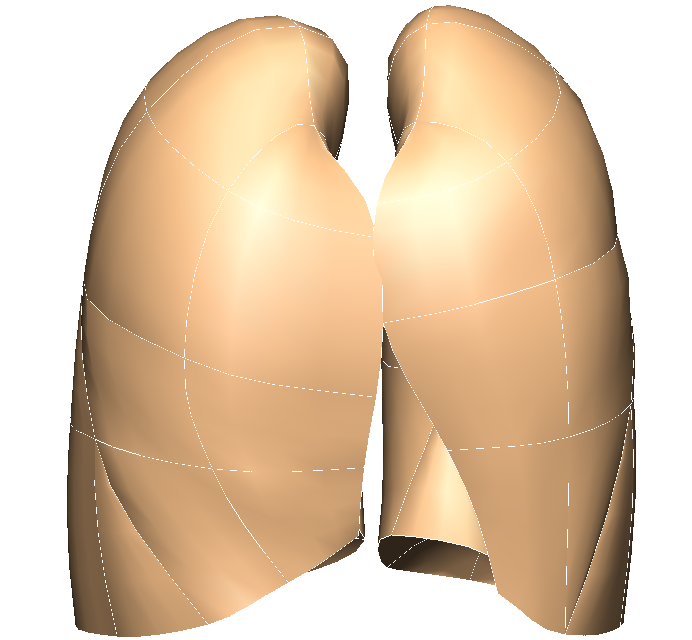
\includegraphics[width=\linewidth,trim={{.0\wd0} {.0\wd0} {.0\wd0} {.0\wd0}},clip]{ModelBasedAnalysis/Image/IPF405_NormalLungMesh.png}
  \caption{Control lung mesh}
  \label{fig:LungShapePrediction-b} 
\end{subfigure}
\caption{Lung mesh for IPF subject and the predicted lung mesh for a normal control with same characteristics. (a) IPF lung mesh generated from CT imaging of a patient with IPF. (b) Control mesh predicted using the reference values for the same patient.}
\label{fig:LungShapePrediction}
\end{figure}

%\begin{table}[htbp]
%\centering
%\caption{Average lobe volume proportion of IPF lung mesh and predicted control lung mesh.}
%\label{tab:AverageLobeVolume_Predicted}
%\begin{tabular}{| l | c | c |}
%\hline
%\bf{Lobe} & \bf{IPF} & \bf{Control} \\
%\hline
%Left lower lobe & 0.231 & 0.242\\
%\hline
%Left upper lobe	& 0.290 & 0.228\\
%\hline
%Right lower lobe	& 0.205 & 0.272\\
%\hline
%Right middle lobe	& 0.130 & 0.078\\
%\hline
%Right upper lobe	& 0.144 & 0.179\\
%\hline
%\end{tabular}
%\end{table} 

\subsection{Construction of airway/vasculature geometry}
\subsubsection{Airway tree}
Figure \ref{fig:AirwayGeometry} illustrates the generated airway trees of one IPF patient and its corresponding predicted airway tree for the control. 

\newgeometry{bottom=2.5cm} %set the left margin of page
\begin{landscape}
\begin{table}[p]
\centering
\caption{Average lobe volume proportion of IPF lung mesh and predicted control lung mesh.}
\label{tab:AverageLobeVolume_Predicted}
\begin{tabular}{| c | c | c | c | c | c | c | c | c | c | c | c |}
%\begin{tabular}{| p{1.2cm} | p{2.2cm} | p{1.0cm} | p{1.0cm} | p{1.0cm} | p{1.0cm} | p{1.0cm} | p{1.0cm} | p{1.0cm} | p{1.0cm} | p{1.0cm} | p{1.0cm} |}
\hline
\multirow{2}*{\bf{Patient No.}} & \multirow{2}*{\bf{Time point}} & \multicolumn{2}{|c|}{\bf{LLL}} & \multicolumn{2}{|c|}{\bf{LUL}} & \multicolumn{2}{|c|}{\bf{RLL}} & \multicolumn{2}{|c|}{\bf{RML}} & \multicolumn{2}{|c|}{\bf{RUL}}\\ 
\cline{3-12}
~ & ~ & Control & IPF & Control & IPF & Control & IPF & Control & IPF & Control & IPF\\
\hline
\multirow{3}*{Patient 1} & Time point 1 & 0.249 & 0.253 & 0.222 & 0.287  & 0.277 & 0.214 & 0.079 & 0.144 & 0.173 & 0.102 \\	
\cline{2-12}
~ & Time point 2 & 0.248 & 0.257 & 0.222 & 0.287  & 0.277 & 0.211 & 0.079 & 0.144 & 0.174 & 0.102 \\
\cline{2-12}
~ & Time point 3 & 0.249 & 0.265 & 0.221 & 0.286  & 0.278 & 0.187 & 0.079 & 0.143 & 0.172 & 0.119 \\
\hline
\multirow{2}*{Patient 2} & Time point 1 & 0.231 & 0.194 & 0.238 & 0.287  & 0.262 & 0.213 & 0.081 & 0.105 & 0.188 & 0.201 \\	
\cline{2-12}
~ & Time point 2 & 0.234 & 0.186 & 0.236 & 0.302  & 0.265 & 0.201 & 0.080 & 0.112 & 0.186 & 0.199 \\
\hline
\multicolumn{2}{|c|}{\bf{Average}} & 0.242 & 0.231 & 0.228 & 0.290  & 0.272 & 0.205 & 0.078 & 0.130 & 0.179 & 0.144 \\
\hline
\end{tabular}
\end{table}
\end{landscape}
\restoregeometry

\newgeometry{bottom=2.5cm} %set the left margin of page
\begin{landscape}
\begin{figure}[htbp]
\begin{subfigure}{7.5cm}
    \makebox[60pt]{\raisebox{50pt}{\rotatebox[origin=c]{0}{\minibox{Control}}}}%
    \sbox0{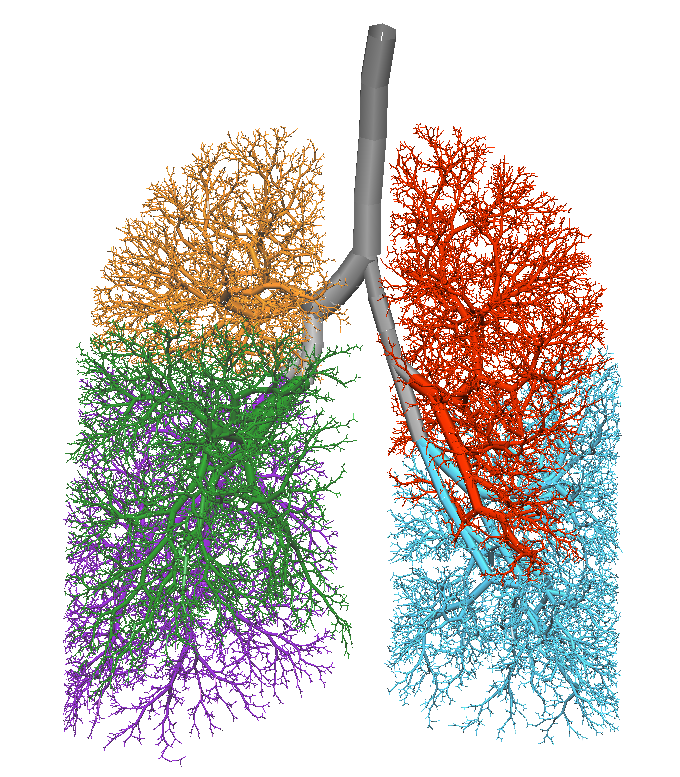
\includegraphics{ModelBasedAnalysis/Image/IPF405_LobeAirway_Normal_1.png}}% get image width, trim={<left> <lower> <right> <upper>}
    \begin{overpic}[height=2.28in,trim={{.0\wd0} {.0\wd0} {.0\wd0} {.0\wd0}},clip]{ModelBasedAnalysis/Image/IPF405_LobeAirway_Normal_1.png}
    \end{overpic}
    \makebox[60pt]{\raisebox{50pt}{\rotatebox[origin=c]{0}{\minibox{IPF}}}}% \makebox:change left space, \raisebox: change upper space
    \begin{overpic}[height=2.03in,trim={{.0\wd0} {.0\wd0} {.0\wd0} {.0\wd0}},clip]{ModelBasedAnalysis/Image/IPF405_LobeAirway_Disease_1.png}
    \end{overpic}
    \caption{Anterior view}
		\label{fig:AirwayGeometry-a}
\end{subfigure}\hspace{0.3cm}
\begin{subfigure}{4.9cm}
    \sbox0{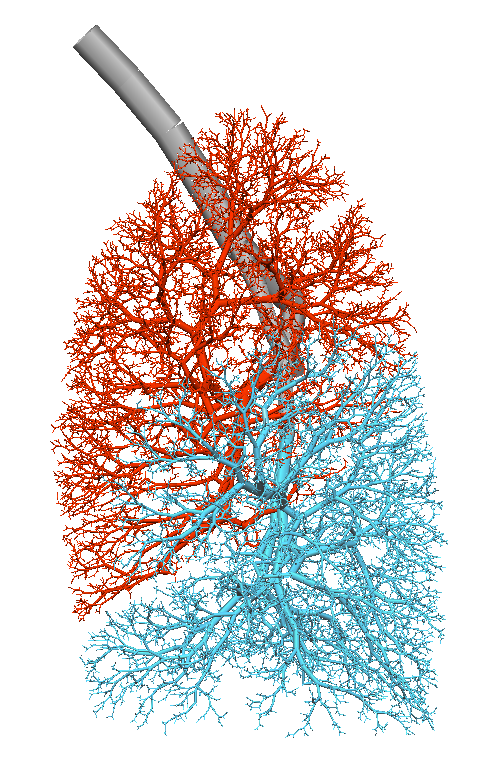
\includegraphics{ModelBasedAnalysis/Image/IPF405_LobeAirway_Normal_2.png}}% get image width, trim={<left> <lower> <right> <upper>}
    \begin{overpic}[height=2.25in,trim={{.0\wd0} {.0\wd0} {.0\wd0} {.0\wd0}},clip]{ModelBasedAnalysis/Image/IPF405_LobeAirway_Normal_2.png}
    \end{overpic}
    \begin{overpic}[height=2.08in,trim={{.0\wd0} {.0\wd0} {.0\wd0} {.0\wd0}},clip]{ModelBasedAnalysis/Image/IPF405_LobeAirway_Disease_2.png}
    \end{overpic}
    \caption{Left lung side}
		\label{fig:AirwayGeometry-b}
\end{subfigure}\hspace{0.3cm}
\begin{subfigure}{4.9cm}
    \sbox0{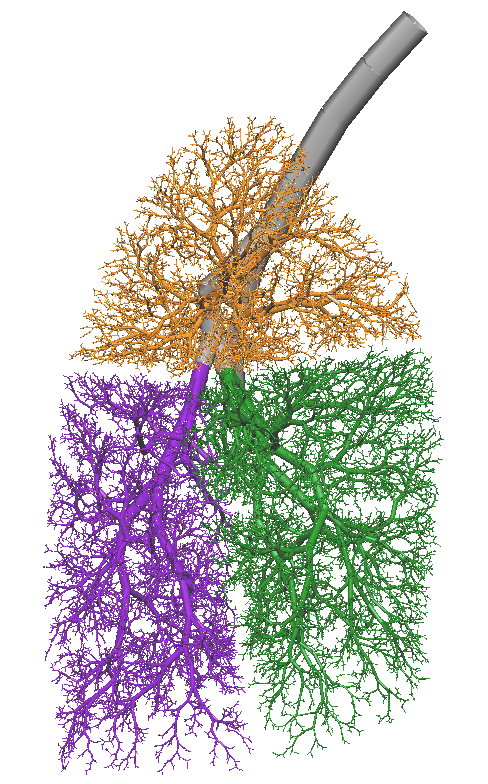
\includegraphics{ModelBasedAnalysis/Image/IPF405_LobeAirway_Normal_3.png}}% get image width, trim={<left> <lower> <right> <upper>}
    \begin{overpic}[height=2.22in,trim={{.0\wd0} {.0\wd0} {.0\wd0} {.0\wd0}},clip]{ModelBasedAnalysis/Image/IPF405_LobeAirway_Normal_3.png}
    \end{overpic}
    \begin{overpic}[height=2.1in,trim={{.0\wd0} {.0\wd0} {.0\wd0} {.0\wd0}},clip]{ModelBasedAnalysis/Image/IPF405_LobeAirway_Disease_3.png}
    \end{overpic}
    \caption{Right lung side}
		\label{fig:AirwayGeometry-c}
\end{subfigure}
\begin{subfigure}{1.7cm}
    \makebox[30pt]{\raisebox{100pt}{\rotatebox[origin=c]{0}{\minibox{\\}}}}
    \sbox0{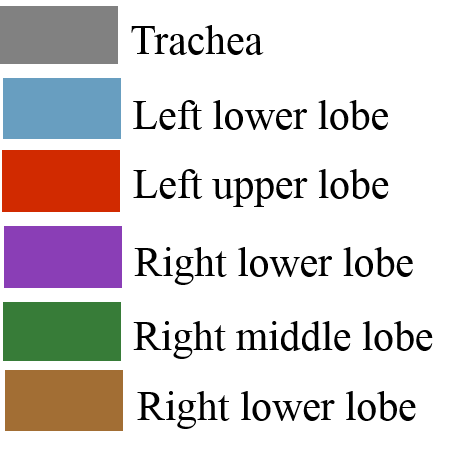
\includegraphics{ModelBasedAnalysis/Image/LobeColors.png}}% get image width, trim={<left> <lower> <right> <upper>}
    \begin{overpic}[height=1.7in,trim={{.0\wd0} {.0\wd0} {.0\wd0} {.0\wd0}},clip]{ModelBasedAnalysis/Image/LobeColors.png}
    \end{overpic}
\end{subfigure}
\caption{Generated normal control airway tree (top row) and IPF airway tree (bottom row) for one patient diagnosed with IPF. (a) Anterior view. (b) Left lung side. (c) Right lung side.}
\label{fig:AirwayGeometry}
\end{figure}
\end{landscape}
\restoregeometry

From Figure \ref{fig:AirwayGeometry}, it can be seen that compared with the control airway tree, the IPF airway tree has a larger trachea radius (which is associated with the dilation of the conducting airway in the IPF lung), a relatively smaller lower lobe and a larger anterior-posterior diameter with respect to the cranio-caudal length. These features are consistent with the SSM based analysis result of IPF lung shape in Chapter 4.

\subsubsection{Vascular tree}
The generated IPF and control artery trees are shown in Figure \ref{fig:VesselTreeGeometry}. Table \ref{tab:AirwayParameter} lists the parameters used for generating the airway tree. Table \ref{tab:VesselParameter} lists the parameters for generating vessel trees. 

\begin{figure}[htbp] 
\centering
\begin{subfigure}{.48\linewidth}% set image scale
  \sbox0{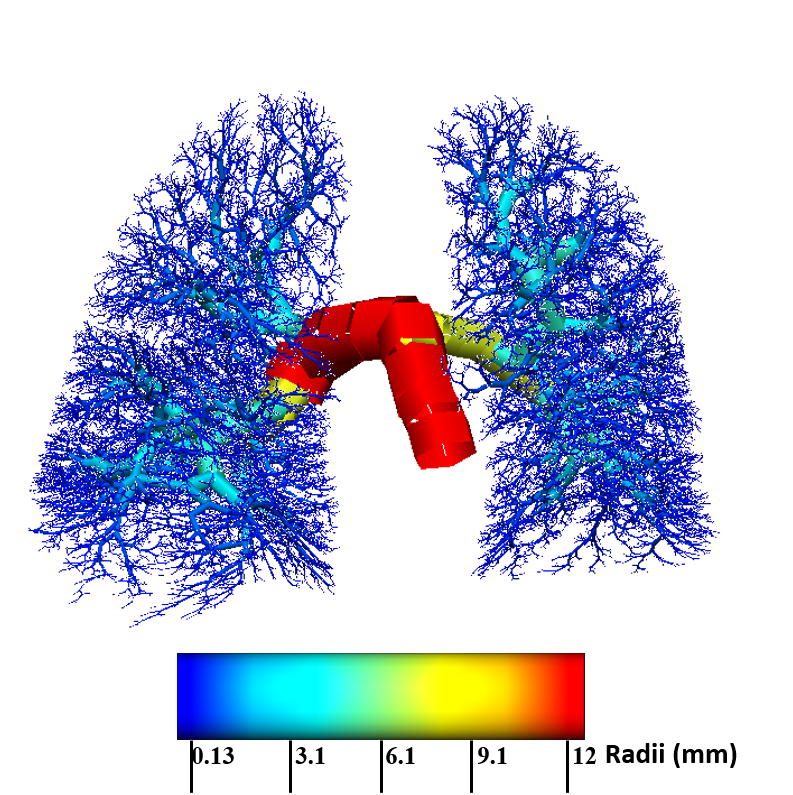
\includegraphics{ModelBasedAnalysis/Image/IPF405_ArteryRadius_IPF.png}}
  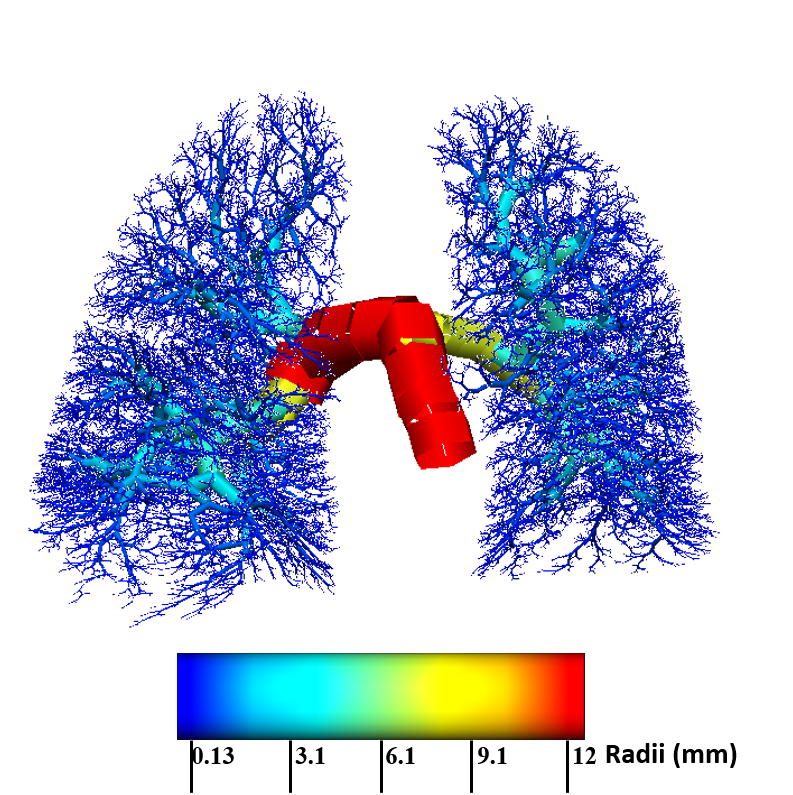
\includegraphics[width=\linewidth,trim={{.0\wd0} {.0\wd0} {.0\wd0} {.0\wd0}},clip]{ModelBasedAnalysis/Image/IPF405_ArteryRadius_IPF.png}
  \caption{IPF vessel tree}
  \label{fig:VesselTreeGeometry-a} 
\end{subfigure}
%\vspace{.1in} % control space between the upper context and figure
\hspace{.1in} % control space between two figures
\begin{subfigure}{.48\linewidth}% set image scale
  \sbox0{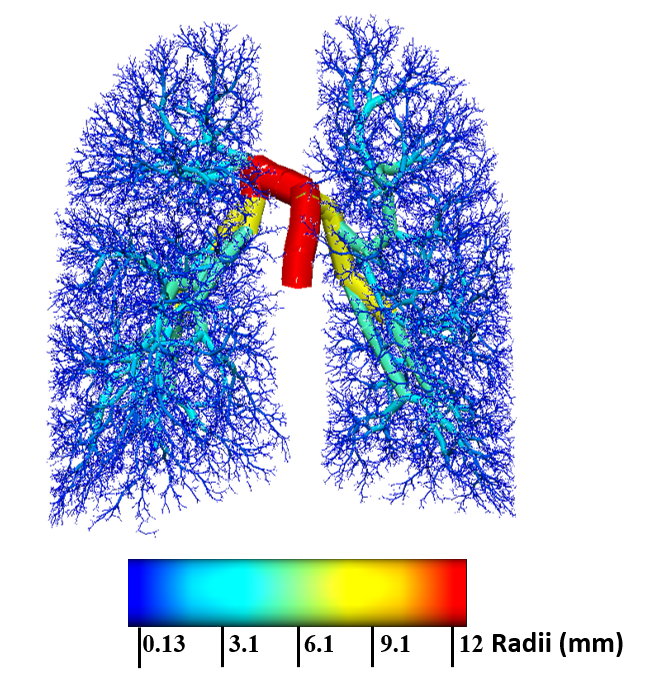
\includegraphics{ModelBasedAnalysis/Image/IPF405_ArteryRadius_Normal.png}}
  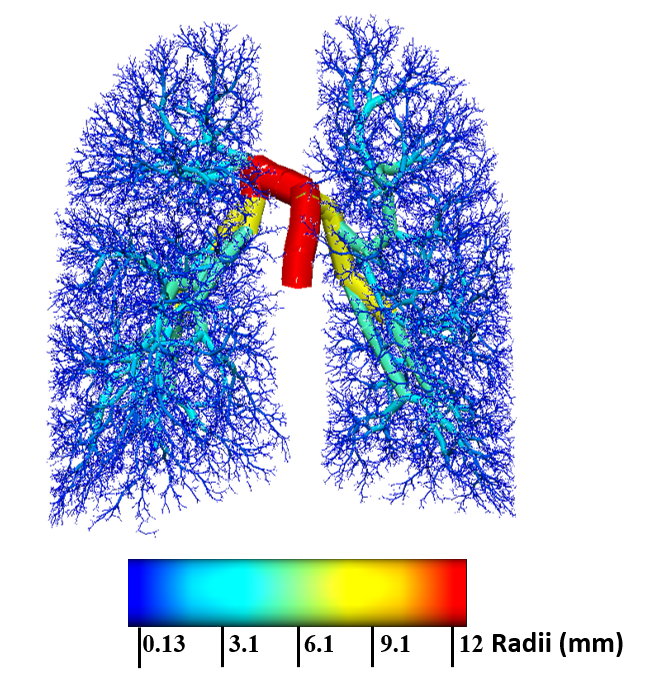
\includegraphics[width=\linewidth,trim={{.0\wd0} {.0\wd0} {.0\wd0} {.0\wd0}},clip]{ModelBasedAnalysis/Image/IPF405_ArteryRadius_Normal.png}
  \caption{Control vessel tree}
  \label{fig:VesselTreeGeometry-b} 
\end{subfigure}
\caption{Generated geometry of the vessel trees. (a) IPF vessel tree. (b) Control vessel tree. The radius of branches are visualized as shown by the colour bars.} 
\label{fig:VesselTreeGeometry}
\end{figure}

\newgeometry{bottom=1.0cm} %set the left margin of page
\begin{landscape}
\begin{table}[p]
\centering
\caption{Parameters of control and IPF airway tree}
\label{tab:AirwayParameter}
\begin{tabular}{| c | c | c | c | c | c | c | c | c | c |}
\hline
\multirow{2}*{\bf{Patient No.}} & \multirow{2}*{\bf{Time point}} & \multicolumn{2}{|c|}{\bf{Trachea radius (mm)}} & \multicolumn{2}{|c|}{\bf{Horsfield diameter ratio($R_dH$})} & \multicolumn{2}{|c|}{\bf{Terminal radius (mm)}} & \multicolumn{2}{|c|}{\bf{Airway volume (ml)}}\\ 
\cline{3-10}
~ & ~ & Normal & IPF & Normal & IPF  & Normal & IPF & Normal & IPF\\
\hline
\multirow{2}*{Patient 1} & Time point 1 & 6.00 & 8.81 & 1.14 & 1.16  & 0.20 & 0.18 & 76.14 & 99.80\\	
\cline{2-10}
~ & Time point 2 & 6.00 & 9.82 & 1.14 & 1.17  & 0.20 & 0.18 & 75.53 & 123.87\\
\cline{2-10}
~ & Time point 3 & 6.00 & 10.03 & 1.14 & 1.16  & 0.20 & 0.18 & 74.17 & 134.84\\
\hline
\multirow{2}*{Patient 2} & Time point 1 & 6.50 & 9.678 & 1.14 & 1.16  & 0.20 & 0.18 & 87.70 & 110.99\\	
\cline{2-10}
~ & Time point 2 & 6.50 & 8.71 & 1.14 & 1.15  & 0.20 & 0.18 & 88.85 & 111.15\\
\hline
\end{tabular}
%\begin{tablenotes}
        %\footnotesize
        %\item{IPF511 and IPF501 are two time points from one patient.}
%\end{tablenotes}
\end{table}

\begin{table}[p]
\centering
\caption{Parameters of control and IPF vessel tree}
\label{tab:VesselParameter}
\begin{tabular}{| c | c | c | c | c | c | c | c | c | c |}
\hline
\multirow{2}*{\bf{Patient No.}} & \multirow{2}*{\bf{Time point}} & \multicolumn{2}{|c|}{\bf{Main artery radius (mm)}} & \multicolumn{2}{|c|}{\bf{Artery $R_dS$}} & \multicolumn{2}{|c|}{\bf{Main vein radius (mm)}} & \multicolumn{2}{|c|}{\bf{Vein $R_dS$}}\\ 
\cline{3-10}
~ & ~ & Normal & IPF & Normal & IPF  & Normal & IPF & Normal & IPF\\
\hline
\multirow{2}*{Patient 1} & Time point 1 & 7.69 & 11.28 & 1.45 & 1.51  & 9.17 & 14.66 & 1.48 & 1.54\\	
\cline{2-10}
~ & Time point 2 & 7.69 & 12.58 & 1.45 & 1.52  & 9.17 & 16.75 & 1.48 & 1.56\\
\cline{2-10}
~ & Time point 3 & 7.69 & 12.86 & 1.45 & 1.52  & 9.17 & 17.20 & 1.48 & 1.56\\			
\hline
\multirow{2}*{Patient 2} & Time point 1 & 8.33 & 12.40 & 1.52 & 1.58  & 11.18 & 18.38 & 1.57 & 1.65\\	
\cline{2-10}
~ & Time point 2 & 8.33 & 11.16 & 1.52 & 1.57  & 11.18 & 16.11 & 1.57 & 1.63\\	
\hline
\end{tabular}
%\begin{tablenotes}
        %\footnotesize
        %\item{IPF511 and IPF501 are two time points from one patient.}
%\end{tablenotes}
\end{table}

\end{landscape}
\restoregeometry

\subsection{Deep inspiration modelling}

Table \ref{tab:InspirationVolume} lists the deep inspiration volumes (from FRC to TLC) for the reference values, simulated, and measured values (from the PFT report). In Table \ref{tab:InspirationVolume}, the simulated inspiration volume (with CT-based abnormality labelling) at all time points for the two patients are higher than the measured values. That is, loss of compliance in the abnormal (fibrosis) regions on the volumetric CT is not sufficient to explain the reduction in inspiration volume from FRC to TLC in the model, except at time point 3 in patient 1.

\begin{table}[htbp]
\centering
\caption{Reference normal, simulated and PFT measured inspiration volume (L).}
\label{tab:InspirationVolume}
\begin{tabular}{| c | c | c | c | c |}
\hline
\bf{Patient No.} & \bf{Time point} & \bf{Ref. normal} & \bf{Simulated} & \bf{PFT measured}\\ 
\hline
\multirow{2}*{Patient 1} & Time point 1 & 1.93 & 1.26 & 1.16\\	
\cline{2-5}
~ & Time point 2 & 1.93 & 1.27 & 1.12 \\
\cline{2-5}
~ & Time point 3 & 1.84 & 1.15 & 1.14\\			
\hline
\multirow{2}*{Patient 2} & Time point 1 & 3.4 & 2.58 & 2.37 \\	
\cline{2-5}
~ & Time point 2 & 3.36 & 2.37 & 1.93 \\	
\hline
\end{tabular}
\end{table}

Additional ''fibrosis'' was added to the CALIPER classified ''normal'' tissues until the modelled inspiration volume matched the measured one (as in the last column of Table \ref{tab:InspirationVolume}). The percentages of CT-based fibrosis (CALIPER classified) and PFT-based fibrosis (CALIPER classified + additional labelled) are listed in Table \ref{tab:FibrosisPercent}. 

%\begin{figure}[H]
  %\centering 
  %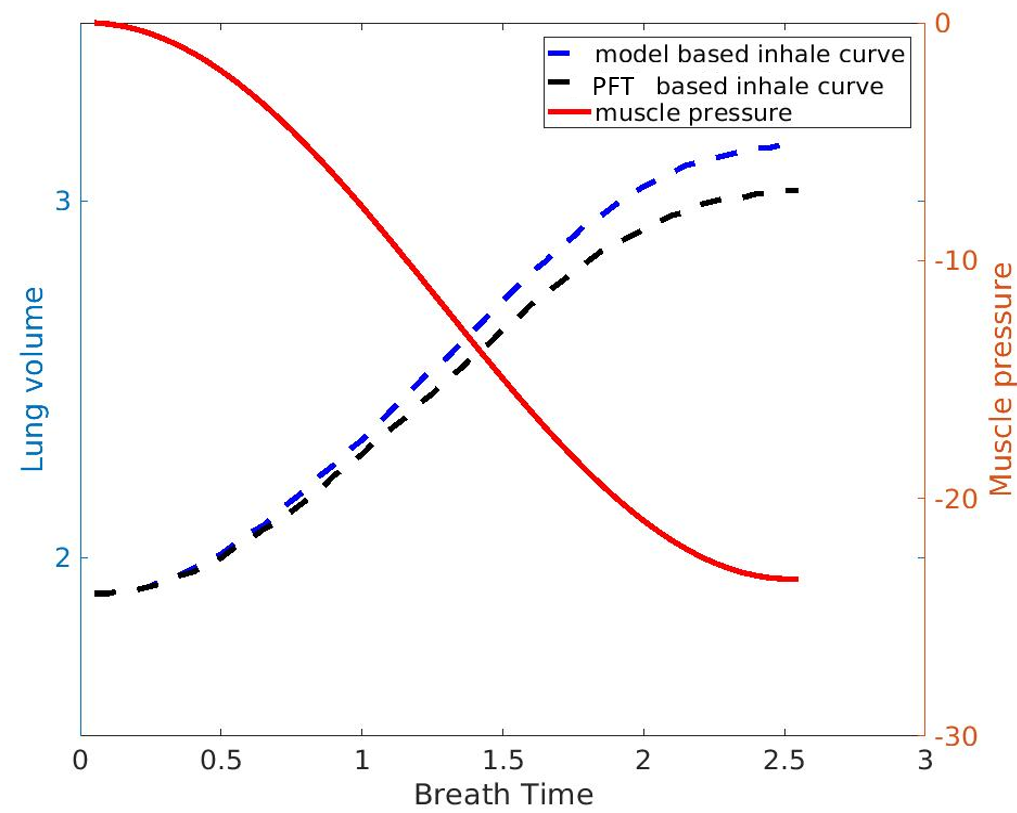
\includegraphics[height=2.9in]{ModelBasedAnalysis/Image/InspirationCurve.png}
  %\caption{Deep inspiration and muscle pressure curve. The red line is the muscle pressure curve. The blue lines is the CT-based simulated inspiration curve with CAPLIPER fibrosis labelled, and red line is the PFT-based simulated inspiration curve with additional fibrosis labelled.}
  %\label{fig:InspirationCurve}
%\end{figure}

\begin{table}[htbp]
\centering
\caption{Percentage of CT-based fibrosis from CALIPER classification and PFT-based fibrosis (CT-based plus additional fibrosis required to limit inspiration from FRC to TLC).}
\label{tab:FibrosisPercent}
\begin{tabular}{| c | c | c | c |}
\hline
\bf{Patient No.} & \bf{Time point} & \bf{CT-based fibrosis (\%)} & \bf{PFT-based fibrosis (\%)}\\ 
\hline
\multirow{2}*{Patient 1} & Time point 1 & 17.6 & 23.7\\	
\cline{2-4}
~ & Time point 2 & 18.9 & 28.9 \\
\cline{2-4}
~ & Time point 3 & 22.1 & 22.9\\			
\hline
\multirow{2}*{Patient 2} & Time point 1 & 4.3 & 11.9\\	
\cline{2-4}
~ & Time point 2 & 12.5 & 29.1\\	
\hline
\end{tabular}
\end{table}

The respiratory system compliance (including the chest wall compliance in parallel with the lung) and the total lung compliance predicted from control, CT-based and PFT-based models for each time point are presented in Table \ref{tab:TotalLungCompliance}. From Table \ref{tab:FibrosisPercent} and \ref{tab:TotalLungCompliance}, the total compliances experience a drop with increasing fibrosis percentage. Total lung compliance decreases to less than half the control value in Patient 1, and about half the control value in Patient 2 in the PFT-based model.

\subsection{Perfusion modelling}

Table \ref{tab:PerfusionResultValues} lists the mean pulmonary artery pressure (mPAP), pulmonary vascular resistance (PVR) and pulmonary blood vessel volume (PVV) of control, CT-based and PFT-based models for each time point of these two patients. From the table, the CT-based model has a consistently lower mPAP value compared with the PFT-based model which has more ''fibrosis'' constriction. That is, there is an increase in mPAP when occluding more small vessels in IPF lungs. For PVV, disease models (both CT-based and PFT-based) have a higher value than the normal control model, but most of the increase in PVV probably comes from the larger pulmonary artery size set for disease vessel models. In spite of this, the PVV of the PFT-based model is also slightly higher compared with the CT-based model. This result is consistent with the observation of \cite{Jacob2016Mortality, Jacob2016Evaluation}, which indicated that an increase in PVV can be seen in lungs with more advanced fibrosis. Moreover, when comparing PFT model with CT model, it can be seen a larger value of PVR, which leads to a dilation of arteries and an increase in PVV.

\newgeometry{bottom=3.0cm} %set the left margin of page
\begin{landscape}
\begin{table}[p]
\centering
\caption{Values of total respiratory system and total lung compliance ($\mathrm{L/cmH_2O}$) of normal control, CT-based and PFT-based modelling results.}
\label{tab:TotalLungCompliance}
\begin{tabular}{| c | c | c | c | c | c | c | c |}
\hline
\multirow{2}*{\bf{Patient No.}} & \multirow{2}*{\bf{Time point}} & \multicolumn{3}{|c|}{\bf{Total respiratory system}} & \multicolumn{3}{|c|}{\bf{Total lung}}\\ 
\cline{3-8}
~ & ~ & \bf{Control} & \bf{CT-based} & \bf{PFT-based} & \bf{Control} & \bf{CT-based} & \bf{PFT-based}\\
\hline
\multirow{2}*{Patient 1} & Time point 1 & 0.108 & 0.070 & 0.064 & 0.235 & 0.108 & 0.094\\	
\cline{2-8}
~ & Time point 2 & 0.108 & 0.070 & 0.060 & 0.235 & 0.108 & 0.086\\
\cline{2-8}
~ & Time point 3 & 0.106 & 0.067 & 0.066 & 0.226 & 0.101 & 0.099\\			
\hline
\multirow{2}*{Patient 2} & Time point 1 & 0.120 & 0.099 & 0.089 & 0.300 & 0.196 & 0.160\\	
\cline{2-8}
~ & Time point 2 & 0.120 & 0.090 & 0.069 & 0.300 & 0.164 & 0.105\\	
\hline
\end{tabular}
\end{table}

\begin{table}[p]
\centering
\caption{Values of mPAP (mmHg), PVR (MPa$\mathrm{\cdot/mm^3}$) and PVV (ml) of normal control, CT-based and PFT-based modelling results.}
\label{tab:PerfusionResultValues}
\begin{tabular}{| c | c | c | c | c | c | c | c | c | c | c |}
\hline
\multirow{2}*{\bf{Patient No.}} & \multirow{2}*{\bf{Time point}} & \multicolumn{3}{|c|}{\bf{mPAP}} & \multicolumn{3}{|c|}{\bf{PVR}} & \multicolumn{3}{|c|}{\bf{PVV}}\\ 
\cline{3-11}
~ & ~ & Control & CT-based & PFT-based & Control & CT-based & PFT-based & Control & CT-based & PFT-based\\
\hline
\multirow{2}*{Patient 1} & Time point 1 & 14.46 & 14.68 & 14.93 & 15.91 & 16.59  & 17.31 & 260.16 & 410.43 & 411.30 \\	
\cline{2-11}
~ & Time point 2 & 14.51 & 14.54 & 14.92 & 15.23 & 15.36 & 16.48 & 260.99 & 550.82 & 552.57 \\
\cline{2-11}
~ & Time point 3 & 14.66 & 14.43 & 14.47 & 17.90 & 17.40 & 17.52 & 272.38 & 583.91 & 584.11 \\
\hline
\multirow{2}*{Patient 2} & Time point 1 & 14.96 & 14.59 & 14.93 & 12.97 & 12.35 & 12.92 & 509.49 & 886.57 & 889.38 \\	
\cline{2-11}
~ & Time point 2 & 14.66 & 15.10 & 16.02 & 12.64 & 13.36 & 14.88 & 515.30 & 798.78 & 804.67 \\
\hline
\end{tabular}
\end{table}
\end{landscape}
\restoregeometry

\subsection{Gas exchange model}
Figure \ref{fig:MainMIGETFigure} illustrates the distribution of control, CT-based and PFT-based simulated V/Q ratio and arterial oxygen at one time point for one IPF patient. The figures are shown with V/Q plotted on a logarithmic scale, which is consistent with the presentation of V/Q measurements using the multiple inert gas elimination technique (MIGET). From the results, the simulation for the control model (the first row) predicts a normal V/Q ratio distribution with $\mathrm{PaO_2}$ of 89.33 mmHg; this slightly low $\mathrm{PaO_2}$ is typical for the normal older adult \citep{wahba1983influence, sprung2006age}. In the control model, most of the alveoli are in the $P_aO_2$ range of 80-100 mmHg. The model labelled with CT-based fibrosis predicts a characteristic (for IPF) bimodal V/Q distribution (the second row), and $\mathrm{PaO_2}$ considerably decreased (71.63 mmHg) from the control. The higher proportion of alveoli appears at high $P_aO_2$ because of the high $\dot{V}$ compared with $\dot{Q}$. It can be observed that about 10\% of alveoli have $P_cO_2$ lower than 63 mmHg which has a net effect of the reduction in total $P_aO_2$. Also, in the CT-based model, there are more low $P_cO_2$ acinus units with relatively high perfusion. A slight shift to the left hand side is observed for the highest peak of the V/Q ratio curve compared with the control model. The smaller peak of the V/Q ratio appears around V/Q = 5 (larger than 1), as there is a decrease in perfusion in fibrotic regions due to the narrowed vessel radius. The model with additional fibrosis (with appropriate patient-specific inspiration from FRC to TLC) predicts further decrease in $\mathrm{PaO_2}$ to 67.85 mmHg. There is an increase in the proportion of well-perfused but less ventilated units, which leads to more alveoli at low $P_cO_2$. Meanwhile, the proportion of ventilation also increases at very high $P_cO_2$ units in the PFT-based model compared with the other two models.

\newgeometry{left=2cm} %set the left margin of page
%\begin{landscape}
\begin{figure}[htbp]
\begin{subfigure}{8.5cm}
    \makebox[60pt]{\raisebox{70pt}{\rotatebox[origin=c]{0}{\minibox{\bf{Normal}}}}}%
    \sbox0{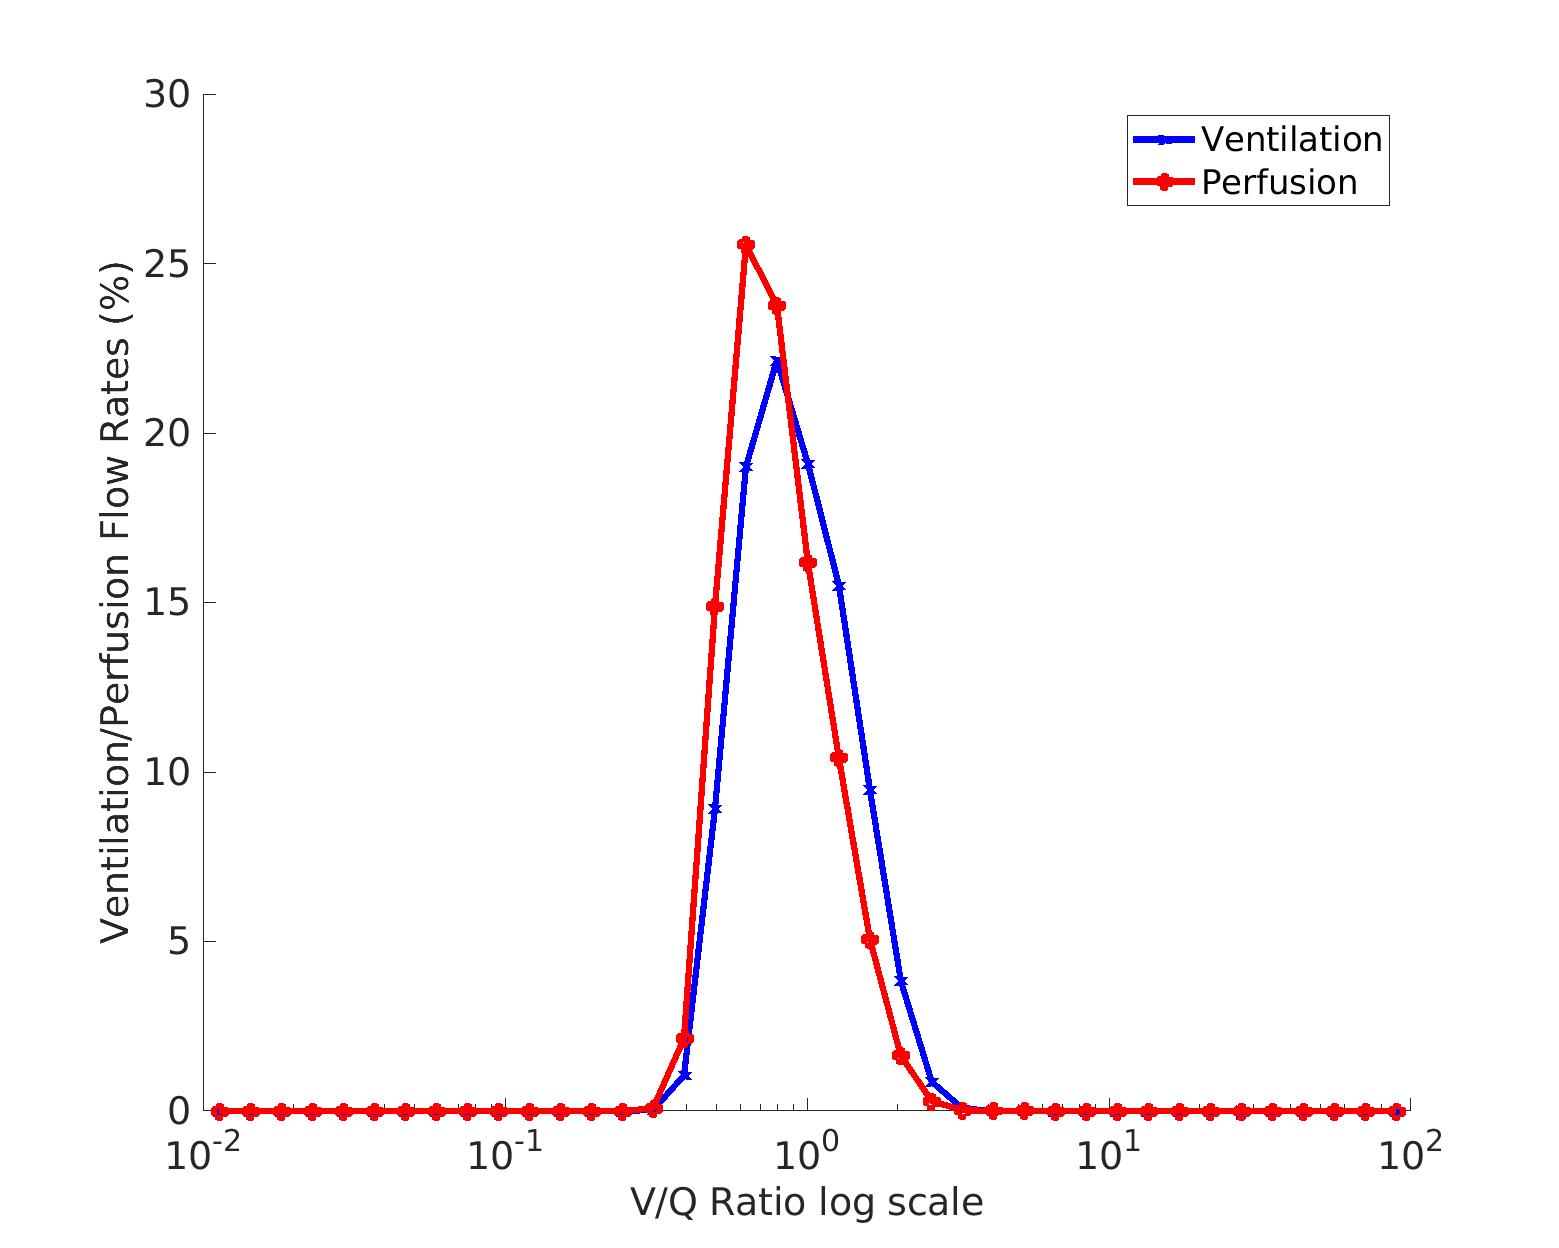
\includegraphics{ModelBasedAnalysis/Image/IPF511_Normal_MIGET_Line_figure.jpg}}% get image width, trim={<left> <lower> <right> <upper>}
    \begin{overpic}[height=2.1in,trim={{.00\wd0} {.00\wd0} {.00\wd0} {.00\wd0}},clip]{ModelBasedAnalysis/Image/IPF511_Normal_MIGET_Line_figure.jpg}
    \end{overpic}
    \makebox[60pt]{\raisebox{70pt}{\rotatebox[origin=c]{0}{\minibox{\bf{CT-based}}}}}% \makebox:change left space, \raisebox: change upper space
    \begin{overpic}[height=2.1in,trim={{.00\wd0} {.00\wd0} {.00\wd0} {.00\wd0}},clip]{ModelBasedAnalysis/Image/IPF511_CTBased_MIGET_Line_figure.jpg}
    \end{overpic}
		\makebox[60pt]{\raisebox{70pt}{\rotatebox[origin=c]{0}{\minibox{\bf{PFT-based}}}}}% \makebox:change left space, \raisebox: change upper space
    \begin{overpic}[height=2.1in,trim={{.00\wd0} {.00\wd0} {.00\wd0} {.00\wd0}},clip]{ModelBasedAnalysis/Image/IPF511_PFTBased_MIGET_Line_figure.jpg}
    \end{overpic}
    \caption{V/Q ratio}
		\label{fig:MainMIGETFigure-a}
\end{subfigure}\hspace{0.3cm}
\begin{subfigure}{9.0cm}
    \sbox0{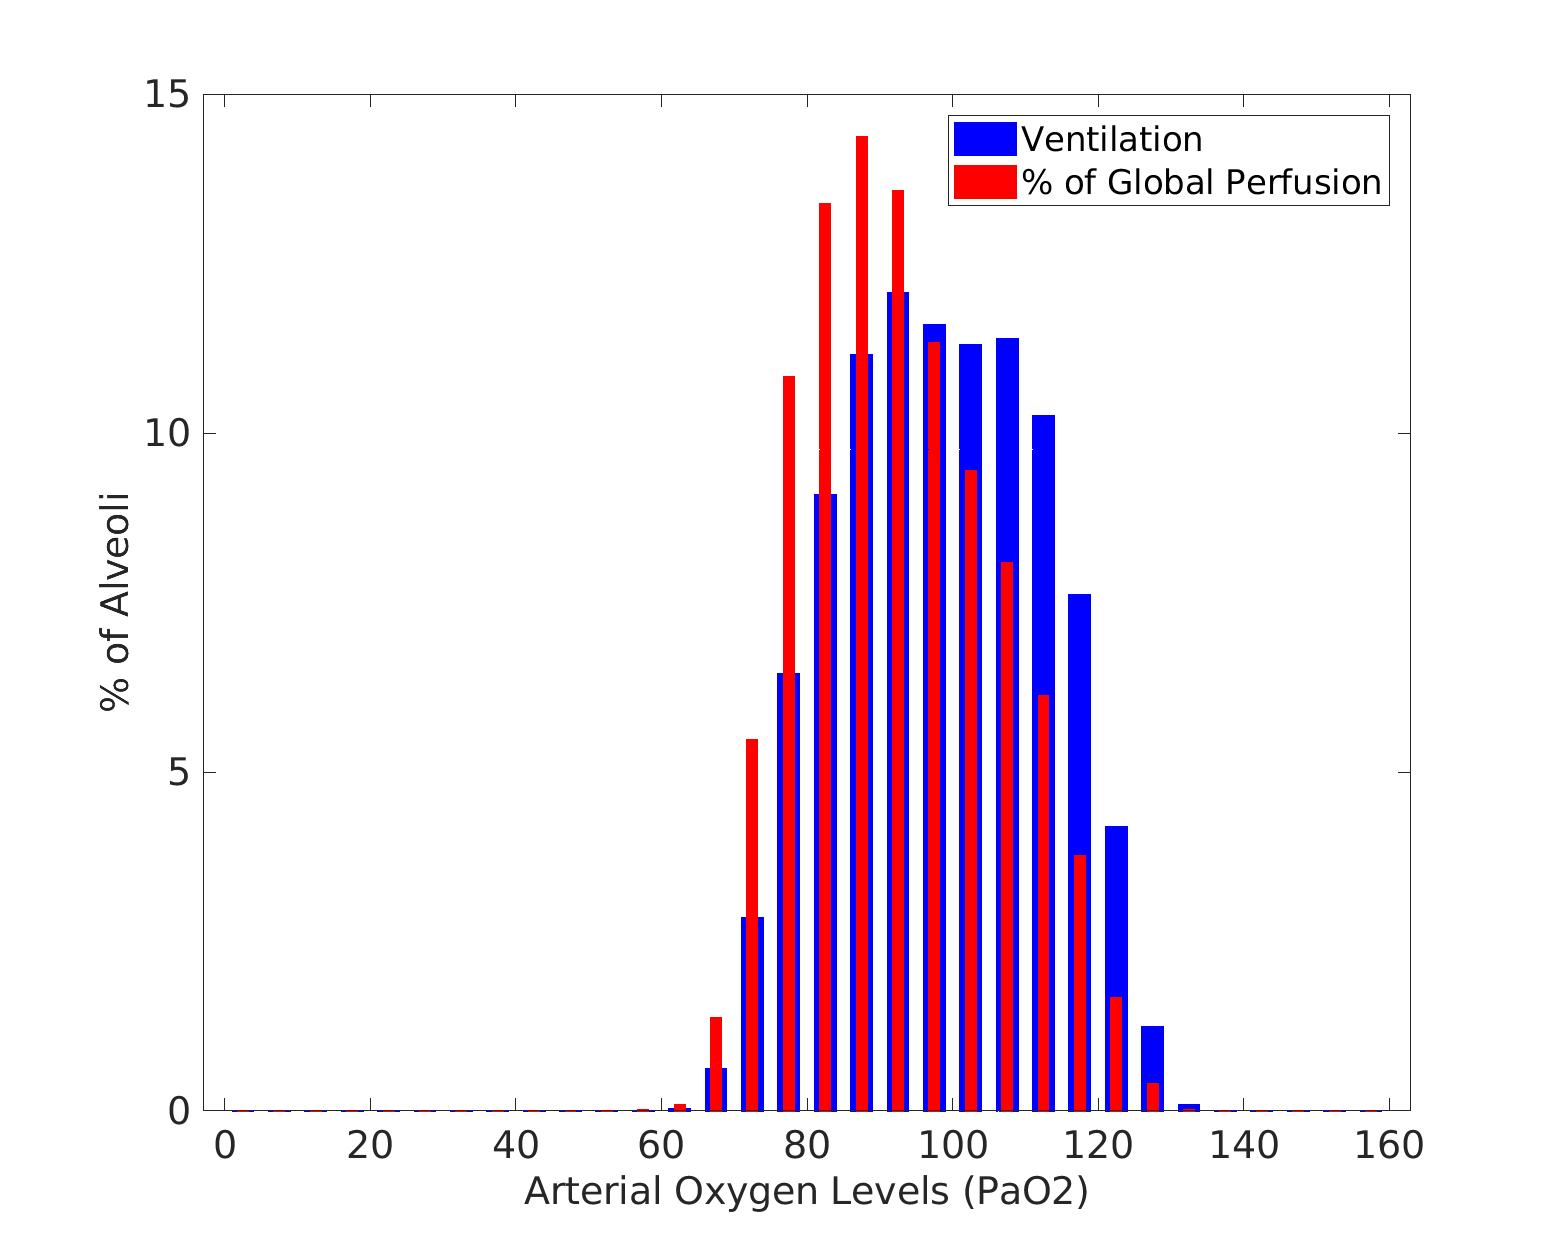
\includegraphics{ModelBasedAnalysis/Image/IPF511_Normal_MIGET_Bar_figure.jpg}}% get image width, trim={<left> <lower> <right> <upper>}
    \begin{overpic}[height=2.1in,trim={{.00\wd0} {.00\wd0} {.00\wd0} {.00\wd0}},clip]{ModelBasedAnalysis/Image/IPF511_Normal_MIGET_Bar_figure.jpg}
    \end{overpic}
    \begin{overpic}[height=2.1in,trim={{.00\wd0} {.00\wd0} {.00\wd0} {.00\wd0}},clip]{ModelBasedAnalysis/Image/IPF511_CTBased_MIGET_Bar_figure.jpg}
    \end{overpic}
    \begin{overpic}[height=2.1in,trim={{.00\wd0} {.00\wd0} {.00\wd0} {.00\wd0}},clip]{ModelBasedAnalysis/Image/IPF511_PFTBased_MIGET_Bar_figure.jpg}
    \end{overpic}
    \caption{End-capillary oxygen level}
		\label{fig:MainMIGETFigure-b}
\end{subfigure}
\caption{V/Q ratio distribution and end-capillary oxygen distribution of control, CT-based and PFT-based simulation result at one time point for one patient diagnosed with IPF). (a) V and Q with respect to V/Q ratio. (b) Distribution of end-capillary oxygen levels amongst alveoli.}
\label{fig:MainMIGETFigure}
\end{figure}
\restoregeometry
%\end{landscape}

Figure \ref{fig:MainVQDistribution} shows the $\dot{V}$, $\dot{Q}$ and V/Q ratio distributions against lung height (cranio-caudal axis) simulated in the control, CT-based and PFT-based models. For the upright models, $\dot{V}$ is higher in the lung base than apex (Figure \ref{fig:MainVQDistribution-a}). The main difference between the control and fibrosis models is a left-wards shift of the $\dot{V}$ curves because of lower total ventilation. The CT- and PFT-based models have very similar $\dot{V}$. Differences in $\dot{Q}$ are mainly in the basal part of the lung, where more fibrosis appears in the fibrosis models. The two fibrosis models have much higher variability of $\dot{Q}$ within iso-gravitational slices (the error bars in Figure \ref{fig:MainVQDistribution-a} and \ref{fig:MainVQDistribution-b}) than the control model, particularly in the basal region. For the control model simulation, V/Q ratio is $\sim$ 1, with a slight increase moving apically.

\begin{figure}[htbp]  
\centering
\begin{subfigure}{.6\linewidth}% set image scale
  \sbox0{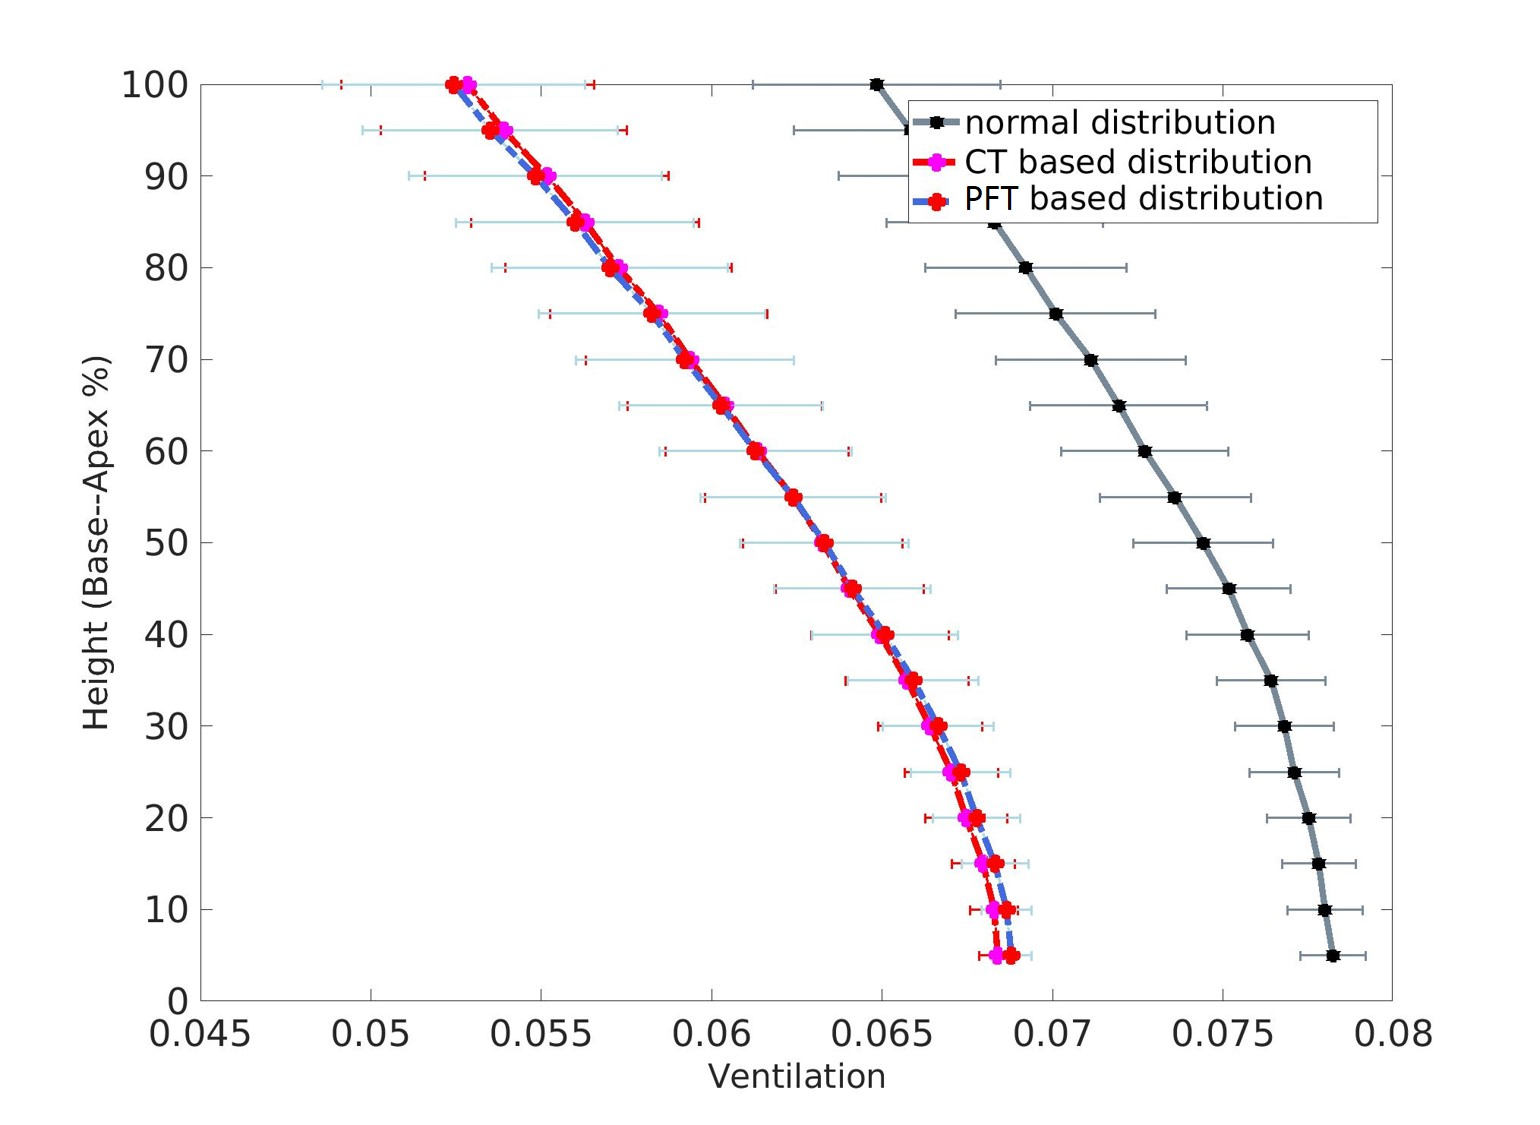
\includegraphics{ModelBasedAnalysis/Image/VentilationAgainstLungHeight.jpg}} 
  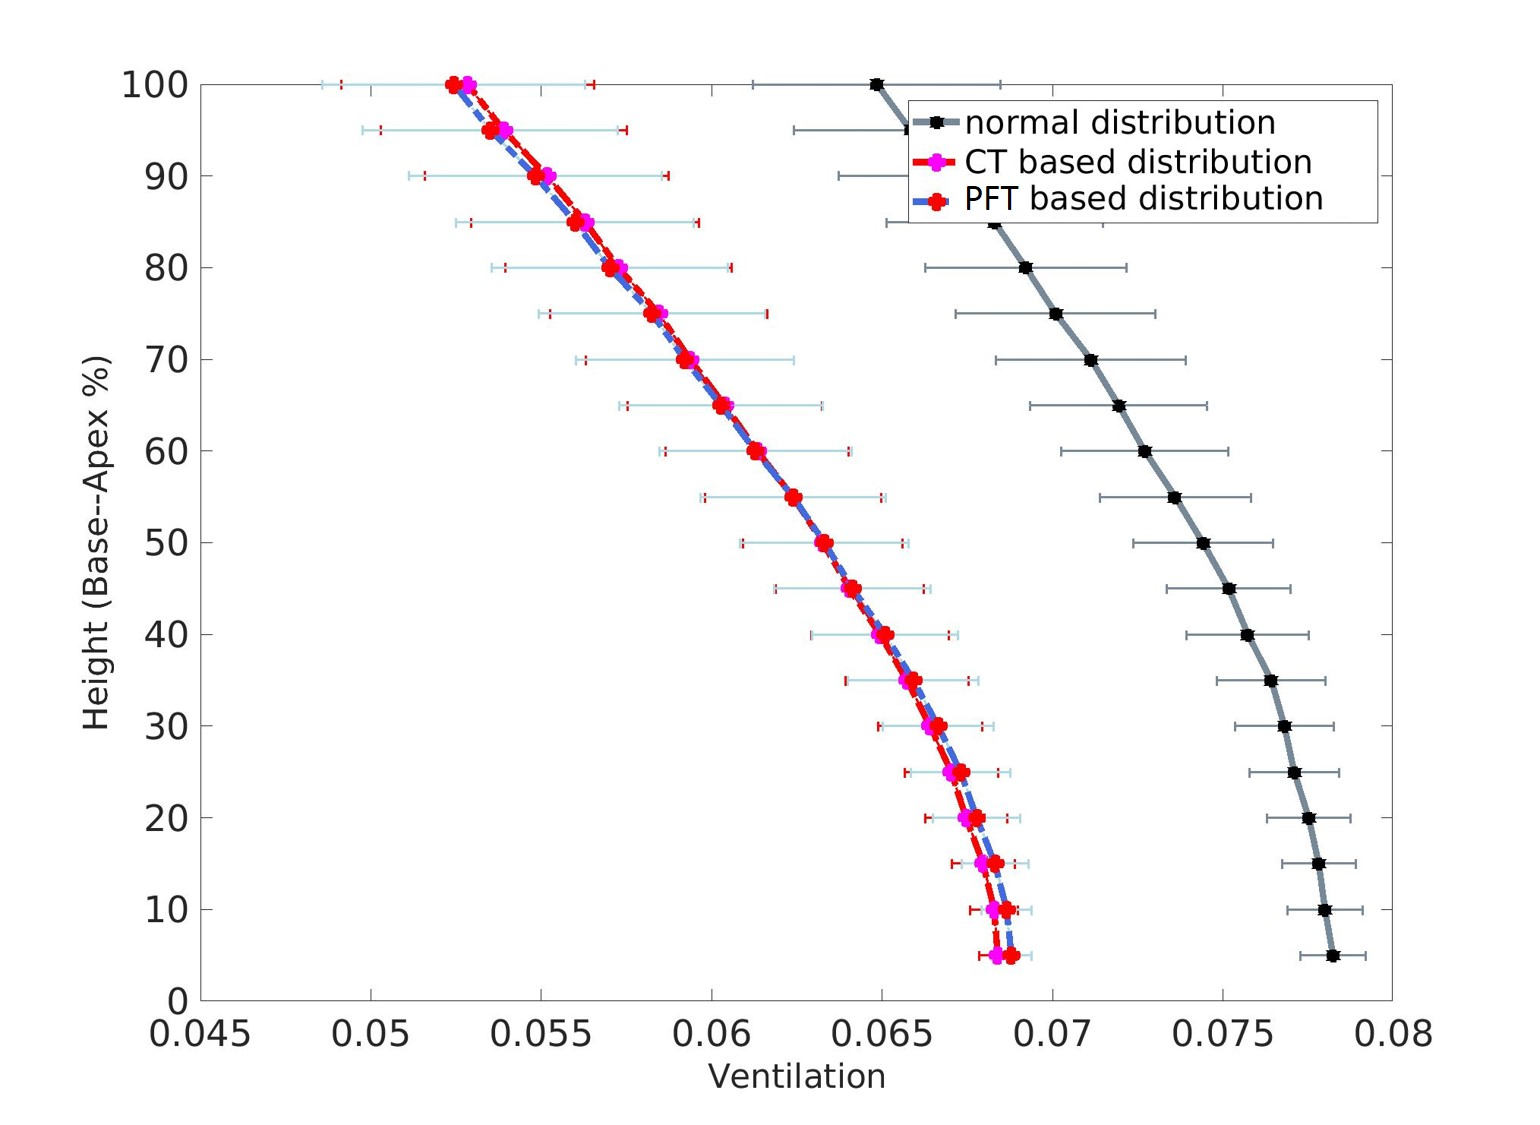
\includegraphics[width=\linewidth,trim={{.0\wd0} {.0\wd0} {.0\wd0} {.0\wd0}},clip]{ModelBasedAnalysis/Image/VentilationAgainstLungHeight.jpg} %trim={<left> <lower> <right> <upper>}, set the cut scale
  \caption{Ventilation distribution}
  \label{fig:MainVQDistribution-a} 
\end{subfigure} 
\begin{subfigure}{.6\linewidth}% set image scale
  \sbox0{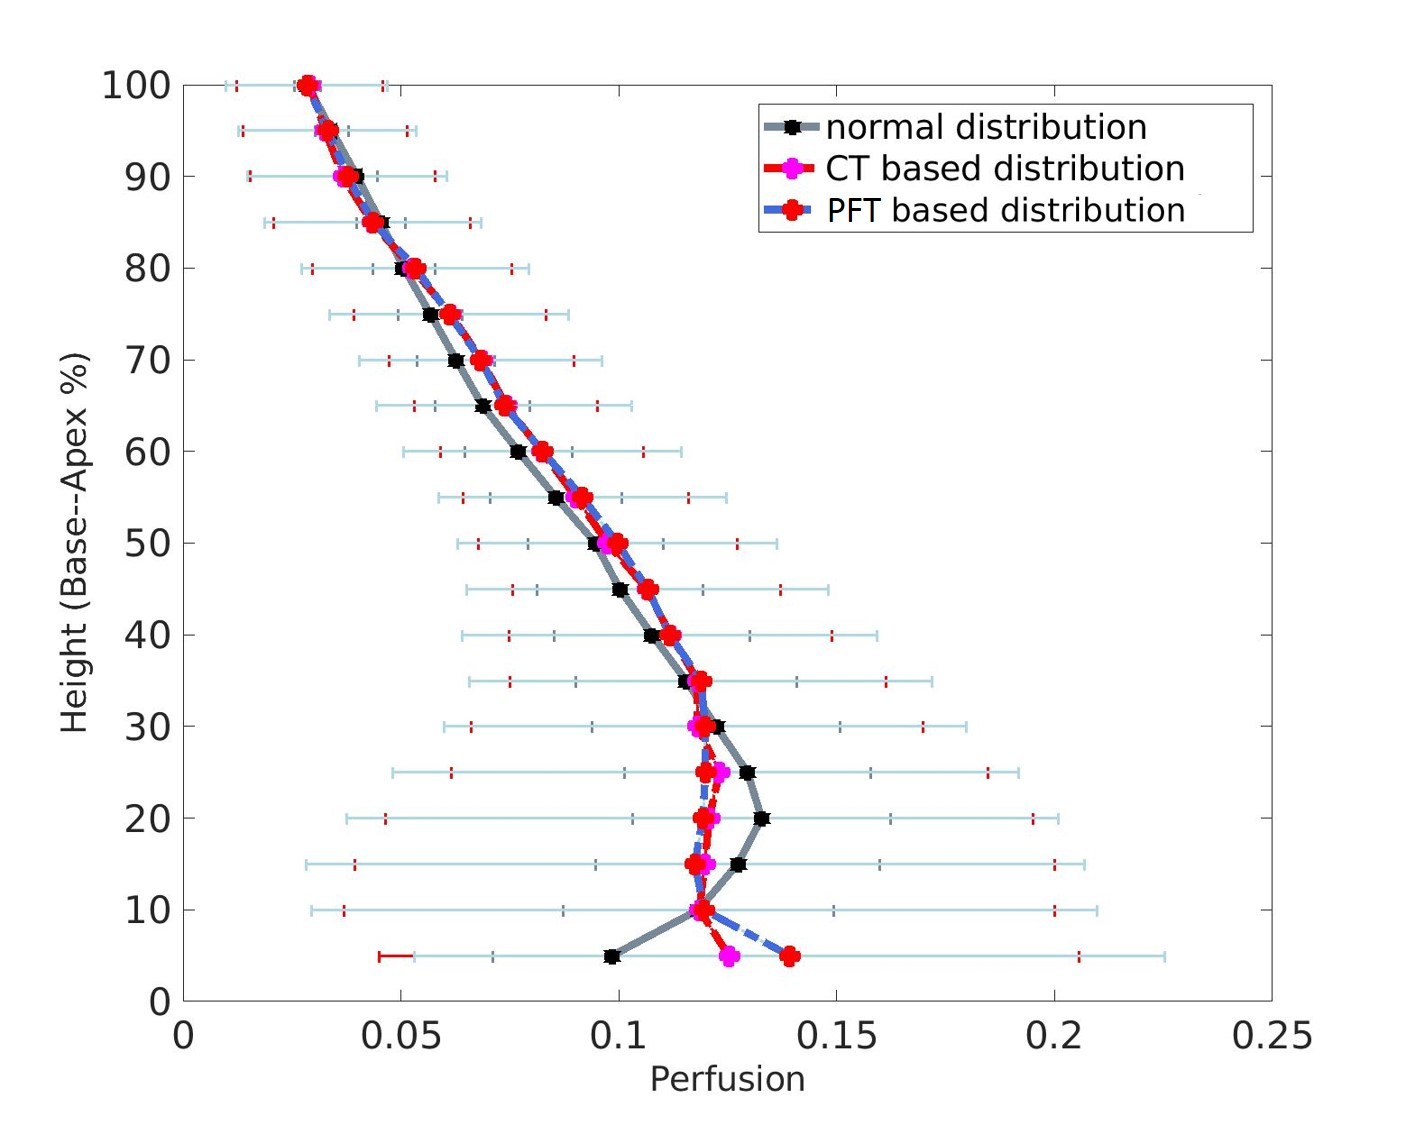
\includegraphics{ModelBasedAnalysis/Image/PerfusionAgainstLungHeight.jpg}}
  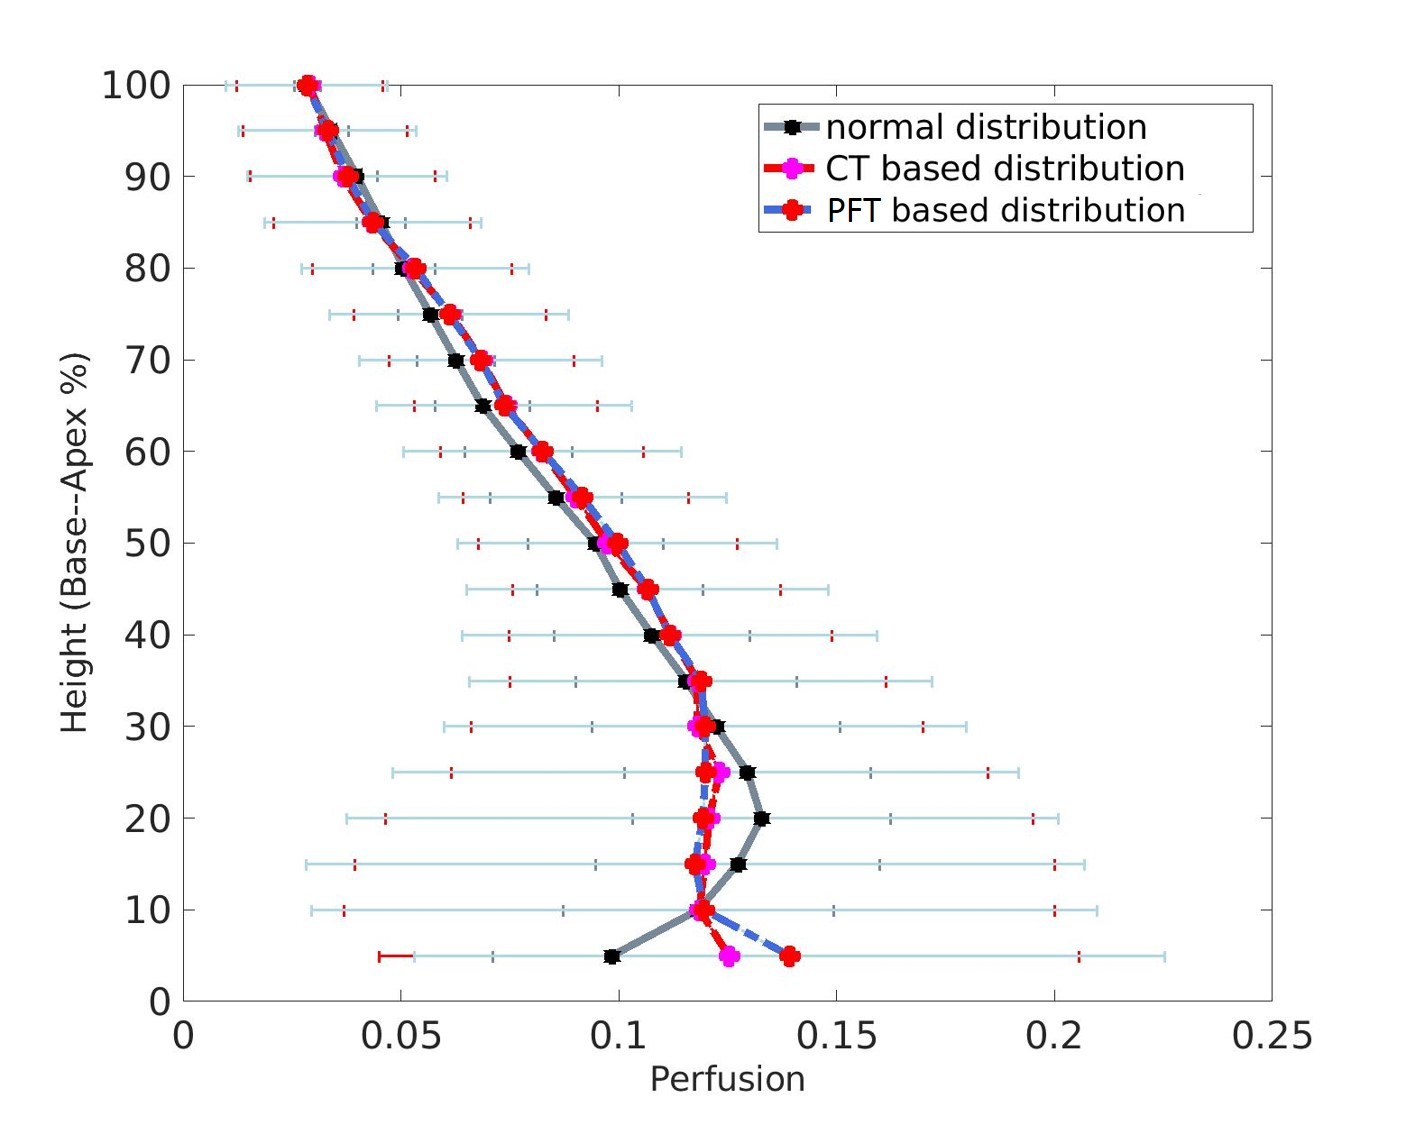
\includegraphics[width=\linewidth,trim={{.0\wd0} {.0\wd0} {.0\wd0} {.0\wd0}},clip]{ModelBasedAnalysis/Image/PerfusionAgainstLungHeight.jpg}
  \caption{Perfusion distribution}
  \label{fig:MainVQDistribution-b}
\end{subfigure}
\begin{subfigure}{.6\linewidth}% set image scale
  \sbox0{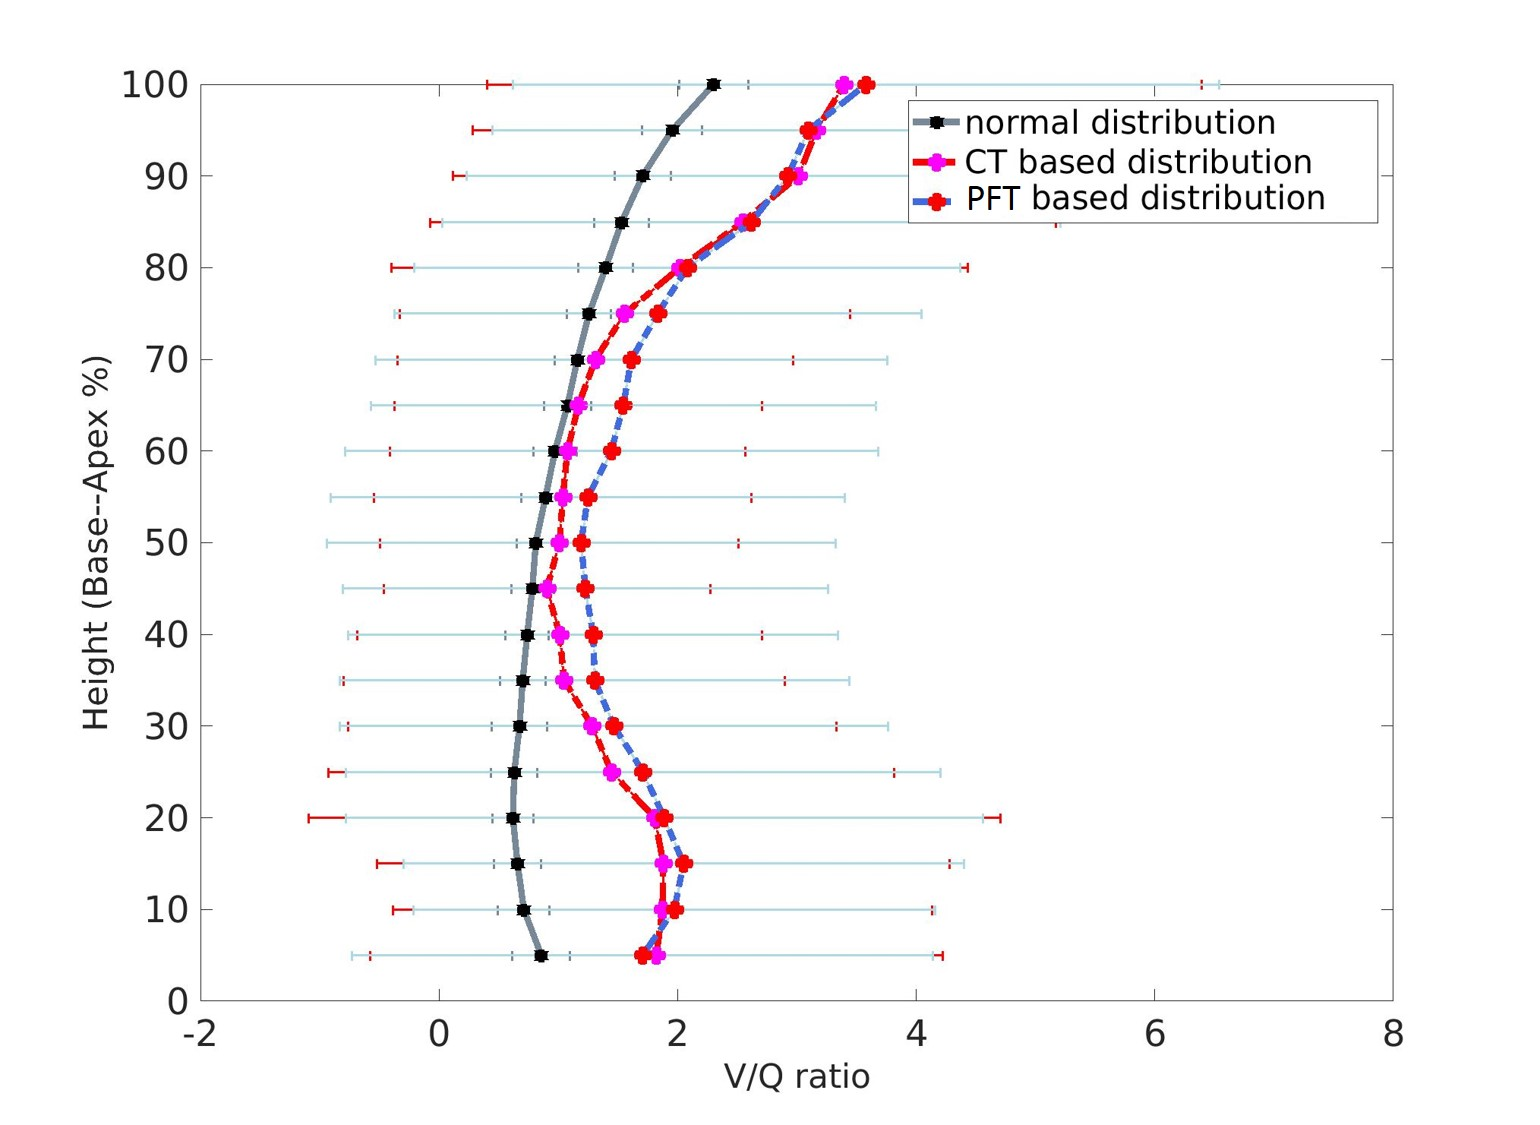
\includegraphics{ModelBasedAnalysis/Image/VQAgainstLungHeight.jpg}}
  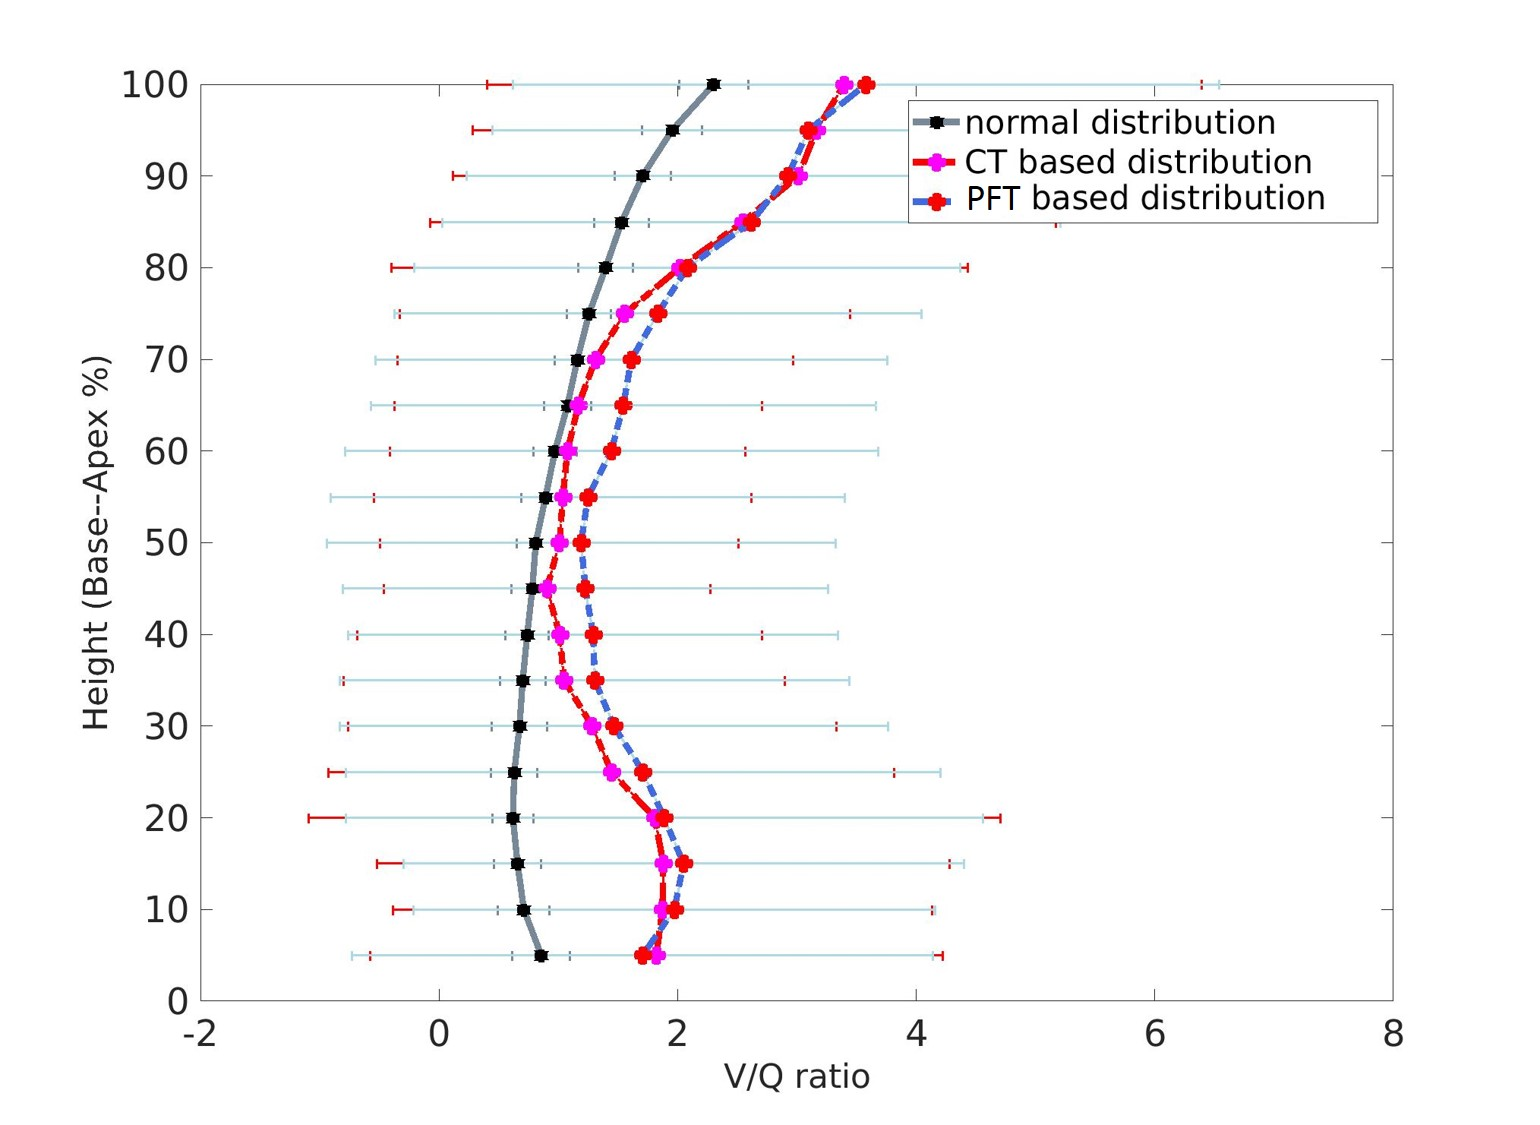
\includegraphics[width=\linewidth,trim={{.0\wd0} {.0\wd0} {.0\wd0} {.0\wd0}},clip]{ModelBasedAnalysis/Image/VQAgainstLungHeight.jpg}
  \caption{V/Q ratio distribution}
  \label{fig:MainVQDistribution-c}
\end{subfigure}
\caption{ Ventilation, perfusion and V/Q ratio distribution against lung height (cranio-caudal axis). (a) Ventilation distribution against lung height. (b) Perfusion distribution against lung height. (c) V/Q ratio distribution against lung height.}
\label{fig:MainVQDistribution}
\end{figure}

The measured DLCO values for each time point of these two patients, and the values of $\mathrm{PaO_2}$ and $\mathrm{PaCO_2}$ for control, CT-based and PFT-based models for each time point are listed in Table \ref{tab:PartialPressure}. For CT-based and PFT-based simulation, $\mathrm{PaO_2}$ experiences an overall decrease over time for both of these two patients, corresponding to the gradual increase of fibrosis. The reduction of $\mathrm{PaO_2}$ and $\mathrm{P(A-a)O_2}$ predicted by the PFT-based model follows the reduction in measured DLCO (and $\mathrm{P(A-a)O_2}$, which has an opposite trend), with the first patient decreasing from time point 1 to time point 2 but slightly increasing from time point 2 to time point 3, and the second patient decreasing from time point 1 to time point 2. MIGET plots of V/Q ratio and arterial oxygen distribution, plots of cranio-caudal distribution of V, Q and V/Q ratio for other subjects and time points can be found in Appendix \ref{appendixMIGET}.

\newgeometry{bottom=1.0cm} %set the left margin of page
\begin{landscape}
\begin{table}[p]
\centering
\caption{Measured DLCO (mL/mmHg/min) for each time point, and values of $\mathrm{PaO_2}$ (mmHg), $\mathrm{PaCO_2}$ (mmHg) and $\mathrm{P(A-a)O_2}$ (mmHg) of normal control, CT-based and PFT-based modelling results.}
\label{tab:PartialPressure}
\begin{tabular}{| c | c | c | c | c | c | c | c | c | c | c | c |}
\hline
\multirow{2}*{\bf{Patient No.}} & \multirow{2}*{\bf{Time point}} & \multirow{2}*{\bf{DLCO}} & \multicolumn{3}{|c|}{\bf{$\mathrm{PaO_2}$}} & \multicolumn{3}{|c|}{\bf{$\mathrm{PaCO_2}$ }} & \multicolumn{3}{|c|}{\bf{$\mathrm{P(A-a)O_2}$}}\\ 
\cline{4-12}
~ & ~ & ~ & Control & CT-based & PFT-based & Control & CT-based & PFT-based & Control & CT-based & PFT-based\\
\hline
\multirow{2}*{Patient 1} & Time point 1 & 11.8 & 89.33 & 71.63 & 67.85 & 41.87  & 52.73 & 53.97 & 8.59 & 17.09 & 20.79\\	
\cline{2-12}
~ & Time point 2 & 9.8 & 95.37 & 64.56 & 58.72 & 37.81  & 57.48 & 59.58 & 7.69 & 18.13 & 23.87\\
\cline{2-12}
~ & Time point 3 & 10.12 & 87.92 & 60.43 & 60.00 & 42.76  & 59.83 & 59.97 & 9.01 & 20.85 & 21.29\\
\hline
\multirow{2}*{Patient 2} & Time point 1 & 16.20 & 92.31 & 88.52 & 85.13 & 39.80  & 41.74 & 42.86 & 9.90 & 10.06 & 13.35\\	
\cline{2-12}
~ & Time point 2 & 14.50 & 91.72 & 83.70 & 75.35 & 39.09  & 43.77 & 46.76 & 9.75 & 14.29 & 22.94\\
\hline
\end{tabular}
\end{table}
\end{landscape}
\restoregeometry

\section{Discussion}
This chapter sets out to determine whether, based on structural parameters, one can use computational models to predict function in the normal older lung, and in individuals with characteristics of IPF lung disease. The models that have been applied in this chapter demonstrate a good prediction of function in the normal older lung, as has been previously assessed in younger adults \citep{tawhai2004ct, swan2012computational, clark2011interdependent}. In the IPF case, model predictions suggest that there must be disease present that is radiologically silent, as mapping disease labelled regions directly to models of lung expansion shows that, in the subjects assessed, the lung of patients is consistently less compliant that the simulated lung. For gas exchange, the IPF models (based on degradation in structure) give reasonable reductions in gas exchange function, solely through V/Q disturbances.

\subsubsection{SSM based lung shape prediction provides a way to compare lung function of IPF patient with older normal people}
An SSM was used to make a prediction of older normal lung shape for each patient. The SSM based lung shape prediction provides a way to make a comparison of the lung function between a patient-specific lung and its corresponding normal equivalent. The patient-specific shape prediction was achieved based on the patient's individual information which shows significant correlations with older normal lung shape, therefore the estimated lung shape is able to represent the statistical lung shape of older normal people as a control group. Through modelling the airway/vessel tree and lung function with the predicted normal lung mesh, it is possible to quantitatively describe the change of respiratory geometry in IPF lung, the decline of lung function, the severity of disease and the prediction of progression. This could be a promising direction for clinical applications in the future.

\subsubsection{Volumetric CT imaging may not provide sufficient information to explain the stiffness of the IPF lung}
The computational modelling in this chapter suggests that radiologically-identified tissue abnormalities from volumetric CT imaging may be not sufficient to explain the increase in lung stiffness and the decline of lung function in IPF patients. Under the assumption that inspiratory muscle pressure does not change in IPF, ascribing only ''abnormal'' tissue to be highly stiffened could not fully explain the reduction in TLC-FRC volume. Additional tissue (up to 10\% in patient 1 and 17\% in patient 2) was required to be stiffened to achieve a correct prediction of volume change from FRC to TLC. The proportion of fibrosis increased in both patients over time, and the additional fibrosis in the PFT model increased this further except for time point 3 in patient 1, where no ''additional'' fibrosis was needed. Total respiratory system compliance was about 30-40\% lower in the IPF models compared with their controls. All models assumed a chest wall compliance of $\mathrm{0.2 L/cm \cdot H_2O}$. Total lung compliance in the control models was higher than the $\mathrm{0.2 L/cm \cdot H_2O}$ expected for the young adult lung, reflecting the higher tissue compliance for these older subjects. Total lung compliance in the two patient models was about half of ''normal'', with the PFT-based models up to 35\% lower compliance than the CT-based models. The method used here to parameterise the compliance of the tissue units assumes that the IPF subject can generate the same driving pressure for inspiration as the control. While the literature suggests that muscle pressure does not change in IPF \citep{de1980inspiratory}, it is possible that the change in lung and chest wall geometry reduces the transfer of the driving pressure to the lung. Regardless, it is reasonable to expect that tissue with normal appearance on CT has already undergoing remodelling that affects its function. Extension of this method and validation in a larger number of subjects could provide an estimate of the proportion of visually normal but functionally abnormal tissue. 

V/Q mismatch (impaired gas exchange) is present in CT-based abnormal tissue as well as in regions that are classified as 'normal'. Additional V/Q mismatch emerges in the PFT-based model due to tissue unit stiffening and artery constriction, which results in a reduction in $P_aO_2$ and increase in $P_aCO_2$. Blood gas data was not available for any subjects in this thesis to compare with the model predictions; however, DLCO reduced over time and was consistent with the model's prediction of gas exchange impairment. Several potential mechanisms have been proposed important in the development of hypoxaemia in IPF: gas exchange barrier thickening, anatomical shunts, and V/Q mismatch. Results from this study suggests that V/Q mismatch in regions of radiologically-identified tissue abnormality (plus additional regions in the PFT-based model) is sufficient to predict a major reduction in $\mathrm{P_aO_2}$. Gas exchange barrier thickening could have an additional effect, however \cite{swan2010multi} showed that gas exchange was more sensitive to changes in tissue elasticity than barrier thickness.

\subsubsection{The predicted ventilation, perfusion and gas exchange distribution can be explained by the background knowledge of IPF}
The physiological alterations in IPF (discussed in Chapter 2, Section \ref{MechanicalAlteration}) are supportive of the modelling results. First, it has been found that IPF disease often results in reduction in total lung compliance (an increase in lung tissue stiffness), and the alterations of total lung compliance in IPF patients appear to be strongly correlated with the degree of lung fibrosis \citep{fulmer1979morphologic,plantier2018physiology}. As should be expected, the total compliance predicted by the ventilation (deep inspiration) model (Table \ref{tab:FibrosisPercent} and \ref{tab:TotalLungCompliance}) decreases with more fibrosis added into the model lung tissues. Second, although the fibrotic tissue is associated with a reduced number of blood vessels \citep{cosgrove2004pigment,ebina2004heterogeneous}, \cite{Jacob2016Mortality, Jacob2016Evaluation} has demonstrated that pulmonary vessel volume (PVV) increases with fibrosis, and can be used as an independent predictor of mortality. Similarly, the predicted PVV in the PFT-based model is higher than the CT-based model, despite having additional vessel occlusions. The larger PVR in the PFT-based model results in slightly higher mPAP which distends the arteries and increases PVV. It should be noted that the assumed tissue tethering pressure (from tissue to blood vessels) was the same in both models. If this were increased in the PFT-based model, it would further increase PVV. In addition, in the perfusion model, the predicted PVV of disease models are higher than the normal control model, but this might is caused by the larger vessel radius assigned to the disease vessel geometry.  Third, the predicted $\mathrm{P_aO_2}$ (which decreases in IPF lung model) and $P_{A-a}O_2$ (increases in the IPF lung model) from the gas exchange model presents a consistent trend with the change of measured DLCO (from PFTs) over time. DLCO is an important index to measure the gas exchange function of the lung, therefore while the simulated $\mathrm{P_aO_2}$ and $P_{A-a}O_2$ cannot be compared directly against data for these subjects, it is reassuring that the model gas exchange follows the DLCO trend. Collection of blood gas data is not standard during lung function testing, whereas measurement of DLCO is. It would therefore be appropriate in future studies to model DLCO (as a surrogate of gas exchange) and compare directly against data. The preliminary outcomes of the modelling framework demonstrated in this chapter suggest that a model-based approach that combines simulation of abnormal mechanics (from FRC to TLC) and gas exchange could be used to  estimate the amount of abnormally-functioning lung tissue that appears radiologically normal. 

\subsubsection{Limitations of modelling procedure}
There are some limitations of the modelling procedure introduced in this chapter. First, in the IPF lung, there is a dilation in trachea, but a constriction in small airway. In this chapter, the trachea radius of normal lung was scaled from the trachea radius of the IPF lung using a statistically measured ratio which represents the conducting airway volume difference between normal and IPF. The main limitation of this method is that the measured ratio may be not accurate enough for all the subjects even though the standard deviation has been taken into consideration here. A potential approach in future work could be to use the change of dead space to tidal volume ratio in IPF lung in the construction of the airway geometry. 

Second, regions of tissue classified as emphysema or low attenuation area (LAA) were not taken into consideration in this model. Although emphysema classified by CAPLIPER only covers a small proportion of the lung (usually less than 1\%), it is believed to have an impact on the deterioration of lung function together with fibrosis in IPF \citep{cottin2005combined, king2011idiopathic, lin2015combined}. LAA (mild, moderate and severe) can account for a sizable proportion of the lung; both emphysema and LAA are associated with air trapping at the end of inspiration \citep{slebos2015air, hoesein2017air}, which will influence the lung volume at FRC and the change of tissue compliance during breathing. Therefore emphysema and LAA should be accounted for in future extensions of this work.

Third, for some end-stage subjects with a large proportion of fibrotic lesion and a small constricted FRC volume, a larger driving pressure may be needed to drive the expansion of the stiffer lung to TLC, because the deep inspiration volume won't be estimated accurately with a ''normal'' driving pressure. For future studies, this could require explicitly modelling the chest wall in normal and IPF subjects, to understand how chest wall shape change affects chest wall mechanics and the pressures developed during deep inspiration.

%%%%%%%%%%%%%%%%%%%%%%%%%%%%%%%%%%%%%%%%%%%%%%%%
\section{Summary}
In this chapter, a preliminary patient-specific computational modelling method was developed to investigate the association between lung structure and lung function in IPF patients. In order to make a comparison between IPF patients and older normal people, an SSM was used to make a prediction of the lung shape of an equivalent older normal for each patient, and the V/Q distribution and gas exchange were then simulated in normal and IPF conditions, respectively, with CALIPER tissue classification data and PFT data as input. The results show that the computational model can predict a reasonable level of abnormality in ventilation, perfusion and gas exchange in the IPF lung, and suggests a predictable difference of lung function between IPF and older normal people based on lung structure. Moreover, the model results suggest tissue based abnormalities do not fully explain the change in lung function in IPF. These preliminary results suggests that a model-based approach could be developed to estimate the amount of ''normal'' appearing tissue with abnormal function, by considering both lung mechanics (expansion from FRC to TLC) and gas exchange.